\documentclass[10pt]{beamer}

%\logo{
\includegraphics[width=.1\textwidth]{logo.jpg}}
\setbeamertemplate{background}{
\includegraphics[height=\paperheight]{logo.jpg}}
\ifx\pdfoutput\undefined
% we are running LaTeX, not pdflatex
\usepackage{graphicx}
\else
% we are running pdflatex, so convert .eps files to .pdf
\usepackage{graphicx}
\usepackage{epstopdf}
\fi
\usepackage{xeCJK}
%\usepackage{fontspec,xunicode,xltxtra}
\setCJKmainfont[BoldFont=SimHei]{KaiTi}
\setCJKmonofont{SimSun}     % 设置缺省中文字体
%\setmainfont[BoldFont=SimHei]{KaiTi}
%\setmonofont{SimSun}     % 设置缺省中文字体
%\usepackage[noindent]{ctex}
\usepackage{amsmath}
\usepackage{multicol}
\usepackage{fontspec}
\usepackage{tikz}  


\setCJKfamilyfont{song}{SimSun}
\newcommand*{\songti}{\CJKfamily{song}}

%\renewcommand{\figurename}{图}

%%--------------------------------------------------------
% NOTE: 1) This is an UNOFFICIAL LaTeX beamer style for 
%           Beihang University.
%       2) This is not exactly a beamer style, rather
%           it contains two LaTeX files to be inserted 
%           in the slides' source file.
%       3) These files are based on Edward Hartley's work
%   <http://www-control.eng.cam.ac.uk/Main/EdwardHartley>
%       4) Complaints or suggestions are always welcome.
%
% Xiaoke Yang (das.xiaoke@hotmail.com)
% Wed 15 Jun 11:02:17 CST 2016
%--------------------------------------------------------


%--------------------------------------------------------
% Set up the Beihang University Colours for use with
% xcolor
%--------------------------------------------------------

% Blue palette
\definecolor{coreBlue}{rgb}{0.14510 0.29020 0.64706} %#254aa5


%%--------------------------------------------------------
% NOTE: 1) This is an UNOFFICIAL LaTeX beamer style for 
%           Beihang University.
%       2) This is not exactly a beamer style, rather
%           it contains two LaTeX files to be inserted 
%           in the slides' source file.
%       3) These files are based on Edward Hartley's work
%   <http://www-control.eng.cam.ac.uk/Main/EdwardHartley>
%       4) Complaints or suggestions are always welcome.
%
% Xiaoke Yang (das.xiaoke@hotmail.com)
% Wed 15 Jun 11:02:17 CST 2016
%--------------------------------------------------------

%--------------------------------------------------------
% Require tikz to do some text positioning
%--------------------------------------------------------
\usepackage{tikz}

%--------------------------------------------------------
% Use Helvetica rather than Computer Modern Sans Serif
% Comment this out if you prefer Computer Modern
%\usepackage{times}
%--------------------------------------------------------
%\usepackage{helvet}

%--------------------------------------------------------
% If you wish to use Arial, and have the winfonts package
% correctly installed uncomment the following to make the
% default sans serif font Arial
%--------------------------------------------------------
%\usepackage{winfonts}
%\usepackage[T1]{fontenc}
%\renewcommand{\sfdefault}{arial}
%--------------------------------------------------------

%--------------------------------------------------------
% Get rid of the navigation bar 
%--------------------------------------------------------
\beamertemplatenavigationsymbolsempty

%--------------------------------------------------------
% Set the files corresponding to the University crests
% here
%--------------------------------------------------------
% Crest with blue text
\newcommand{\beihangcrestblack}{beihangbeamerstyle/Tongji1.png}

% Crest with white text
%\newcommand{\beihangcrestwhite}{beihangbeamerstyle/beihang-rev-pantone}
%--------------------------------------------------------

%--------------------------------------------------------
% Define how the page counter will be displayed on slides
%--------------------------------------------------------
\newcommand{\footlinepagecounter}%
	{\insertframenumber{}/\inserttotalframenumber}
%--------------------------------------------------------

%--------------------------------------------------------
% Set up some lengths
%--------------------------------------------------------
% A paper width for the footline
\newlength{\halfpaperwidth}

% The left margin
\newlength{\headingleftmargin}
% Paper width minus margins
\newlength{\headingwidthminusmargins}
% Height of the heading block
\newlength{\headingheight}
% Height of the footer block
\newlength{\footerheight}

% The height for the titlepageheader in the title page
\newlength{\titlepageheaderheight}
% The height for the footer in the title page
\newlength{\titlepagefooterheight}
% The height for the main title block
\newlength{\titlepagemaintitleblockheight}
% The height for the subtitle block
\newlength{\titlepagesubtitleblockheight}
% The height for the name and date block
\newlength{\titlepagenamedateblockheight}
% The height for the institution block
%\newlength{\titlepageinstitutionheight}

% The lengths for spacing between name and date
\newlength{\titlepagespaceundername}
\newlength{\titlepagespaceunderdate}

% The length for the light blue thin bar


\setlength{\headingleftmargin}{0.05573\paperwidth}
\setlength{\headingwidthminusmargins}{\paperwidth}
\addtolength{\headingwidthminusmargins}{-\headingleftmargin}
\setlength{\headingheight}{0.1459\paperheight}
\setlength{\footerheight}{0.09017\paperheight}

\setlength{\titlepageheaderheight}{0.2361\paperheight}
\setlength{\titlepagefooterheight}{0.1459\paperheight}
\setlength{\titlepagemaintitleblockheight}{0.2361\paperheight}
\setlength{\titlepagesubtitleblockheight}{0.1459\paperheight}
\setlength{\titlepagenamedateblockheight}{0.2361\paperheight}
%\setlength{\titlepageinstitutionheight}{0.95cm}

\setlength{\titlepagespaceundername}{16pt}
\setlength{\titlepagespaceunderdate}{8pt}

%--------------------------------------------------------

%--------------------------------------------------------
% Set up the Beihang University blue scheme for use
% with beamer
%--------------------------------------------------------

% Define colour names
\setbeamercolor{coreBlue}{bg=coreBlue, fg=white}

% Set element colours
\setbeamercolor{subtitle}{fg=white}
\setbeamercolor{titlepageheader}{bg=white,fg=black}
\setbeamercolor{titlepagefooter}{bg=white,fg=black}
\setbeamercolor{block title}{bg=white, fg=coreBlue}
\setbeamercolor{structure}{bg=white, fg=coreBlue}
% \setbeamercolor{alerted text}{fg=darkOrange}


%--------------------------------------------------------
% Set font sizes
%--------------------------------------------------------
\setbeamerfont{frametitle}{size=\large,series=\bfseries}
\setbeamerfont{title}{size=\large,series=\bfseries}
\setbeamerfont{author}{size=\normalsize}
\setbeamerfont{date}{size=\scriptsize}
\setbeamerfont{subtitle}{size=\footnotesize,series=\bfseries}
\setbeamerfont{block title}{size=\normalsize,series=\bfseries}
\setbeamerfont{structure}{size=\normalsize,series=\bfseries}

\setbeamertemplate{itemize item}{\scriptsize\raise1.25pt\hbox{\textbullet}}
\setbeamertemplate{itemize subitem}{\scriptsize\raise1.25pt\hbox{\textbullet}}
\setbeamertemplate{itemize subsubitem}{\scriptsize\raise1.25pt\hbox{\textbullet}}


%-----------------------------------------------------
% Define frame title drawing
%-----------------------------------------------------
\setbeamertemplate{frametitle}
{%
  \nointerlineskip
  \begin{beamercolorbox}[wd=\paperwidth,leftskip=\headingleftmargin]{coreBlue}
    \vskip1pt%
    \tikz{\node[minimum height=\headingheight, inner sep=0cm, text width= \headingwidthminusmargins, text badly ragged]{\usebeamerfont{frametitle}\insertframetitle\\\normalsize\it\insertframesubtitle};}
  \end{beamercolorbox}%
}

%-----------------------------------------------------
% Define footline drawing
%-----------------------------------------------------
\setbeamertemplate{footline}
{%
 \setlength{\halfpaperwidth}{0.5\paperwidth}
 \addtolength{\halfpaperwidth}{1pt}
 \leavevmode
 \begin{beamercolorbox}[sep=0pt,wd=\paperwidth, leftskip=\headingleftmargin,right]{coreBlue}
 \tikz{\node[minimum height=\footerheight, inner sep=0.2cm]{\footlinepagecounter};}%
 \end{beamercolorbox}
 %\hskip-1.5pt%
 %\begin{beamercolorbox}[sep=0pt,wd=\halfpaperwidth, leftskip=\headingleftmargin,right]{coreBlue}
  %\tikz{\node[minimum height=\footerheight, inner sep=0cm]{\footlinepagecounter};}%
  %\end{beamercolorbox}
 %\begin{beamercolorbox}[sep=0pt,wd=\halfpaperwidth, leftskip=\headingleftmargin, right,rightskip=\headingleftmargin]{coreBlue}
 %\tikz{\node[minimum height=\footerheight, inner sep=0cm]{\includegraphics[width=0.25\paperwidth]{\beihangcrestwhite}};}%
 %\end{beamercolorbox}%
}


%-----------------------------------------------------
% Define BEIHANG title page
%-----------------------------------------------------
\setbeamertemplate{title page}
{%
\begin{beamercolorbox}[sep=0cm,right,wd=\paperwidth,ht=\titlepageheaderheight,rightskip=\headingleftmargin]{titlepageheader}
\includegraphics[width=0.3820\paperwidth]{\beihangcrestblack}
\vskip0.2361\titlepageheaderheight
\end{beamercolorbox}
\begin{beamercolorbox}[left,leftskip=\headingleftmargin,wd=\paperwidth,ht=\titlepagemaintitleblockheight]{coreBlue}
\tikz{\node[inner sep=0cm, text width=\paperwidth, minimum height=\titlepagemaintitleblockheight,text badly ragged]{\usebeamerfont{title}\inserttitle};}%
\end{beamercolorbox}%
\nointerlineskip%
\vskip-1pt%
\begin{beamercolorbox}[left,leftskip=\headingleftmargin,wd=\paperwidth,ht=\titlepagesubtitleblockheight]{coreBlue}
\tikz{\node[inner sep=0cm, text width=\paperwidth, minimum height=\titlepagesubtitleblockheight, text badly ragged]{\usebeamerfont{subtitle}\usebeamercolor[fg]{subtitle}\insertsubtitle};}%
\end{beamercolorbox}%
\nointerlineskip%
\vskip-1pt%
\begin{beamercolorbox}[left,leftskip=\headingleftmargin,wd=\paperwidth,ht=\titlepagenamedateblockheight]{coreBlue}
      \usebeamerfont{author}\insertauthor\\
      \vskip\titlepagespaceundername%
      \usebeamerfont{date}\insertdate
      \vskip\titlepagespaceunderdate%
    \end{beamercolorbox}%
\begin{beamercolorbox}[left,leftskip=\headingleftmargin,wd=\paperwidth,ht=\titlepagefooterheight]{titlepagefooter}
\end{beamercolorbox}
}


\title{\Large 上海市优秀毕业生答辩}
\date{致远楼108, 2019.5.13}
\author{胡雨宽$\quad$1553396\\
\small 同济大学 数学科学学院\\
\small 2015级理科班$\:\:$数学与应用数学}

\AtBeginSection[]
{
  \begin{frame}<beamer>
    \frametitle{提纲}
    \tableofcontents[sections={2-},currentsection,subsectionstyle=show/show/hide]%,sections={2-6}]
  \end{frame}
  \addtocounter{framenumber}{-1}
}

\AtBeginSubsection[]
{
  \begin{frame}<beamer>
    \frametitle{提纲}
    \tableofcontents[sections={2-},currentsection,subsectionstyle=show/shaded/hide]
  \end{frame}
  \addtocounter{framenumber}{-1}
}

\begin{document}
%----------------------------------------------------------------------
% Title frame
\begin{frame}[plain]
\maketitle
\end{frame}

%----------------------------------------------------------------------
% Outline frame
% PLEASE RUN pdflatex TWICE 
\section*{提纲}
\begin{frame}
\frametitle{提纲}
\tableofcontents[sections={2-},hideallsubsections]
\end{frame}
%%=====================================================================
% Section I
%\section{个人简介}
%----------------------------------------------------------------------
% Content frame
%\begin{frame}
%\frametitle{个人简介}
%\begin{columns}
%			\begin{column}{0.4\textwidth}
%				\centering
%				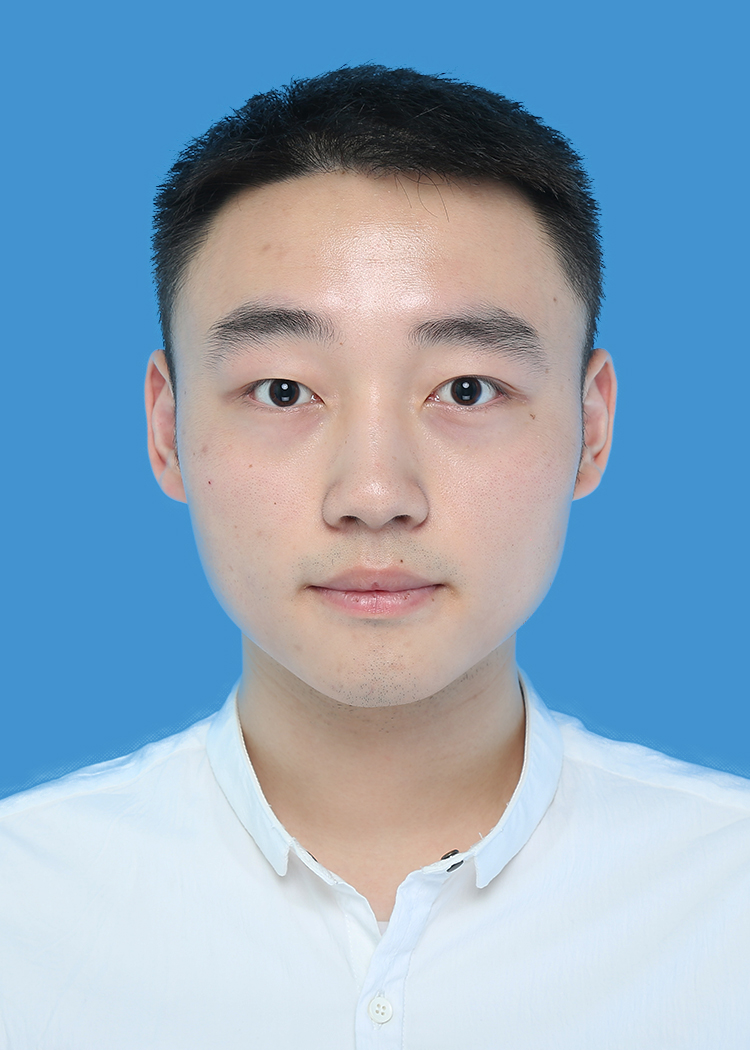
\includegraphics[height = .7\textwidth]{photo.jpg}
%			\end{column}
%			\begin{column}{.6\textwidth}
%				\begin{itemize}
%					\item 姓名: 胡雨宽
%					\item 性别: 男
%					\item 班级: 2015级理科班
%					\item 籍贯: 江西南昌
%				\end{itemize}
%			\end{column}
%\end{columns}
%\end{frame}

%%=====================================================================
% Section II
\section{学习方面}
%----------------------------------------------------------------------
\begin{frame}
\frametitle{学习方面——锐意进取$\,$开拓创新}
%\begin{columns}
%\begin{column}{0.3\textwidth}
%\only<2>{
%\begin{center}
%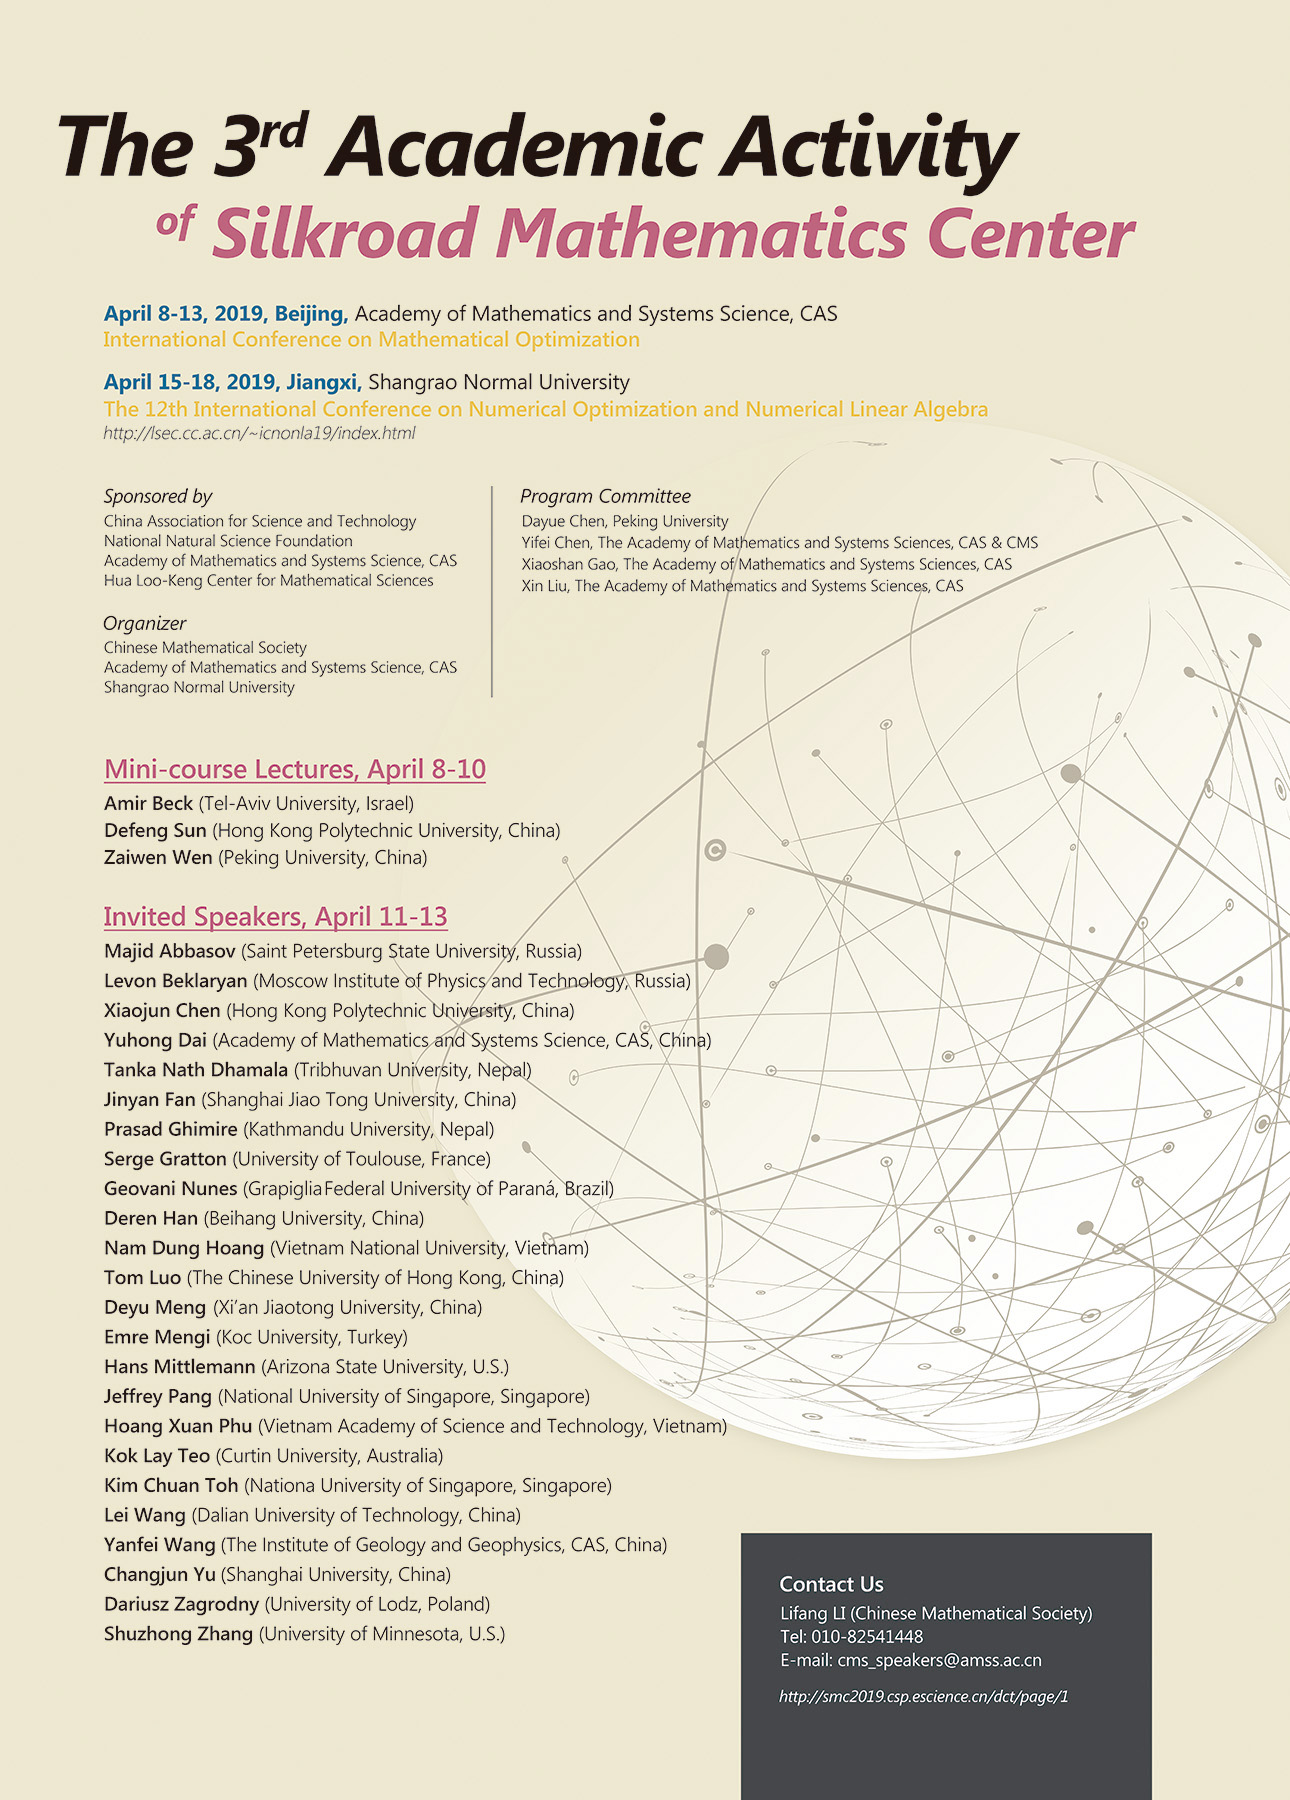
\includegraphics[width=.2\paperwidth]{Silkroad.jpg}\\
%\footnotesize \textbf{图}1: 丝路数学中心第3次学术活动\end{center}}
%\only<3>{\begin{center}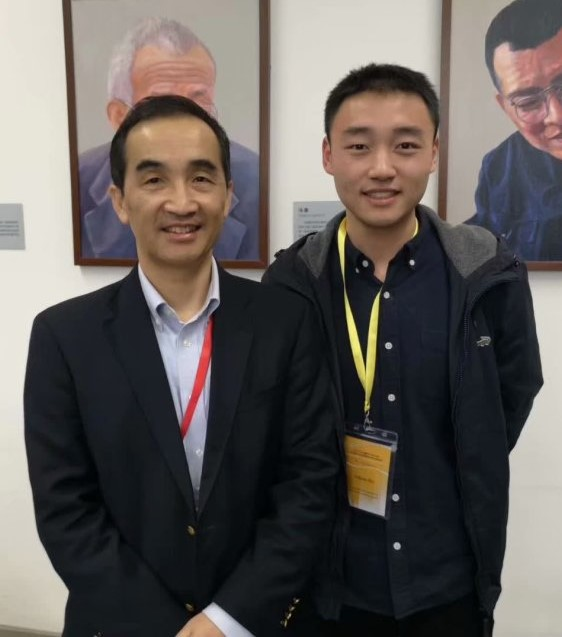
\includegraphics[width=.23\paperwidth]{Silkroadphoto.jpg}\\
%\footnotesize \textbf{图}2: 与香港中文大学(深圳)副校长罗智泉教授的合影\end{center}}
%\only<4>{
%\begin{center}
%\begin{tikzpicture}
%  \node (img1) {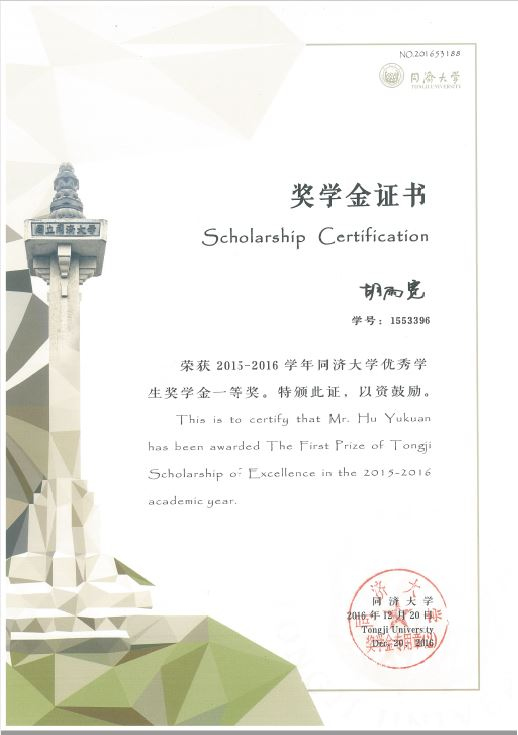
\includegraphics[height=3cm]{15-16一等奖.jpg}};
%  \node (img2) at (img1.south east) {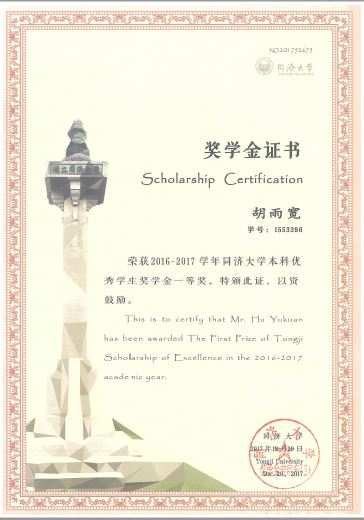
\includegraphics[height=3cm]{16-17一等奖.jpg}};
%\end{tikzpicture}
%\footnotesize \textbf{图}3: 奖学金证书\end{center}}
%\only<5>{
%\begin{center}
%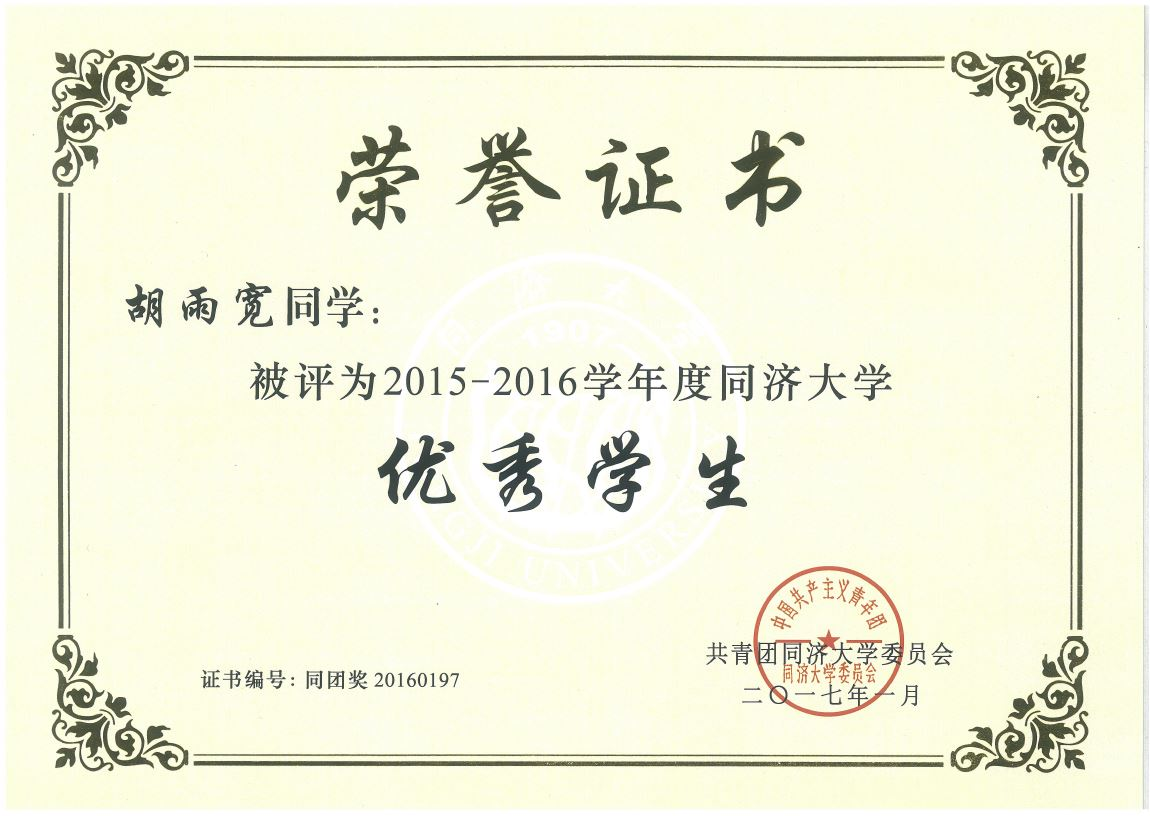
\includegraphics[height=2cm]{15-16优秀学生.jpg}\\
%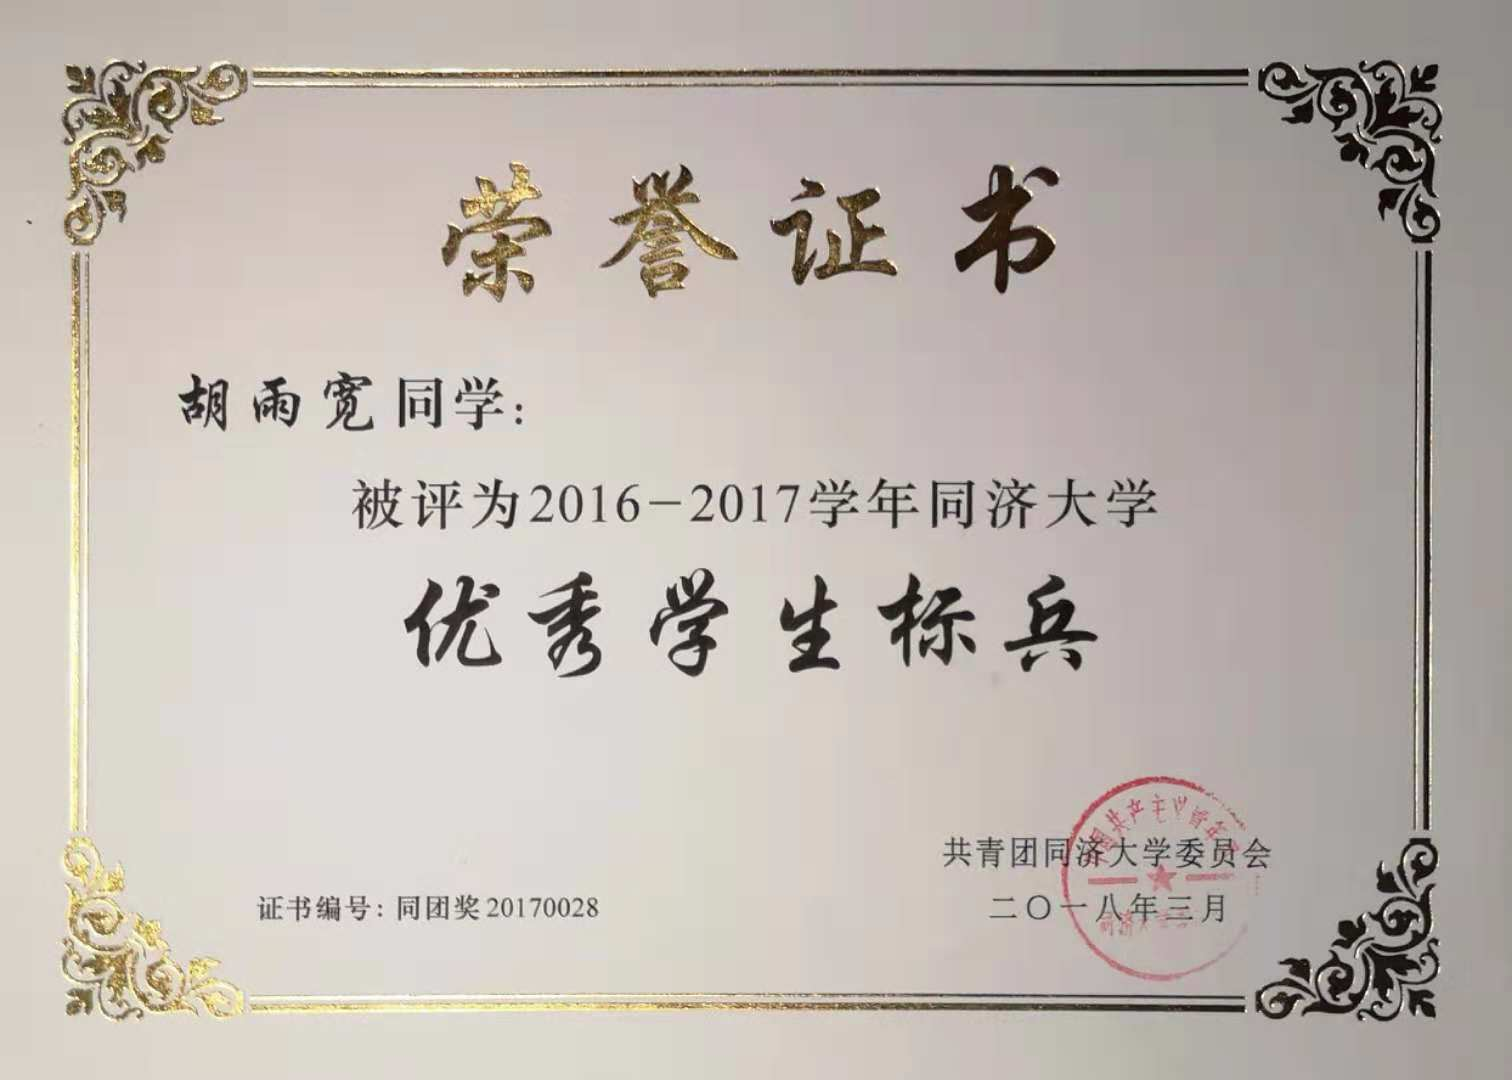
\includegraphics[height=2cm]{16-17优秀学生标兵.jpg}\\
%\footnotesize \textbf{图}4: 优秀学生证书
%\end{center}
%}
%\only<6>{
%\begin{center}
%\begin{tikzpicture}
%  \node (img1) {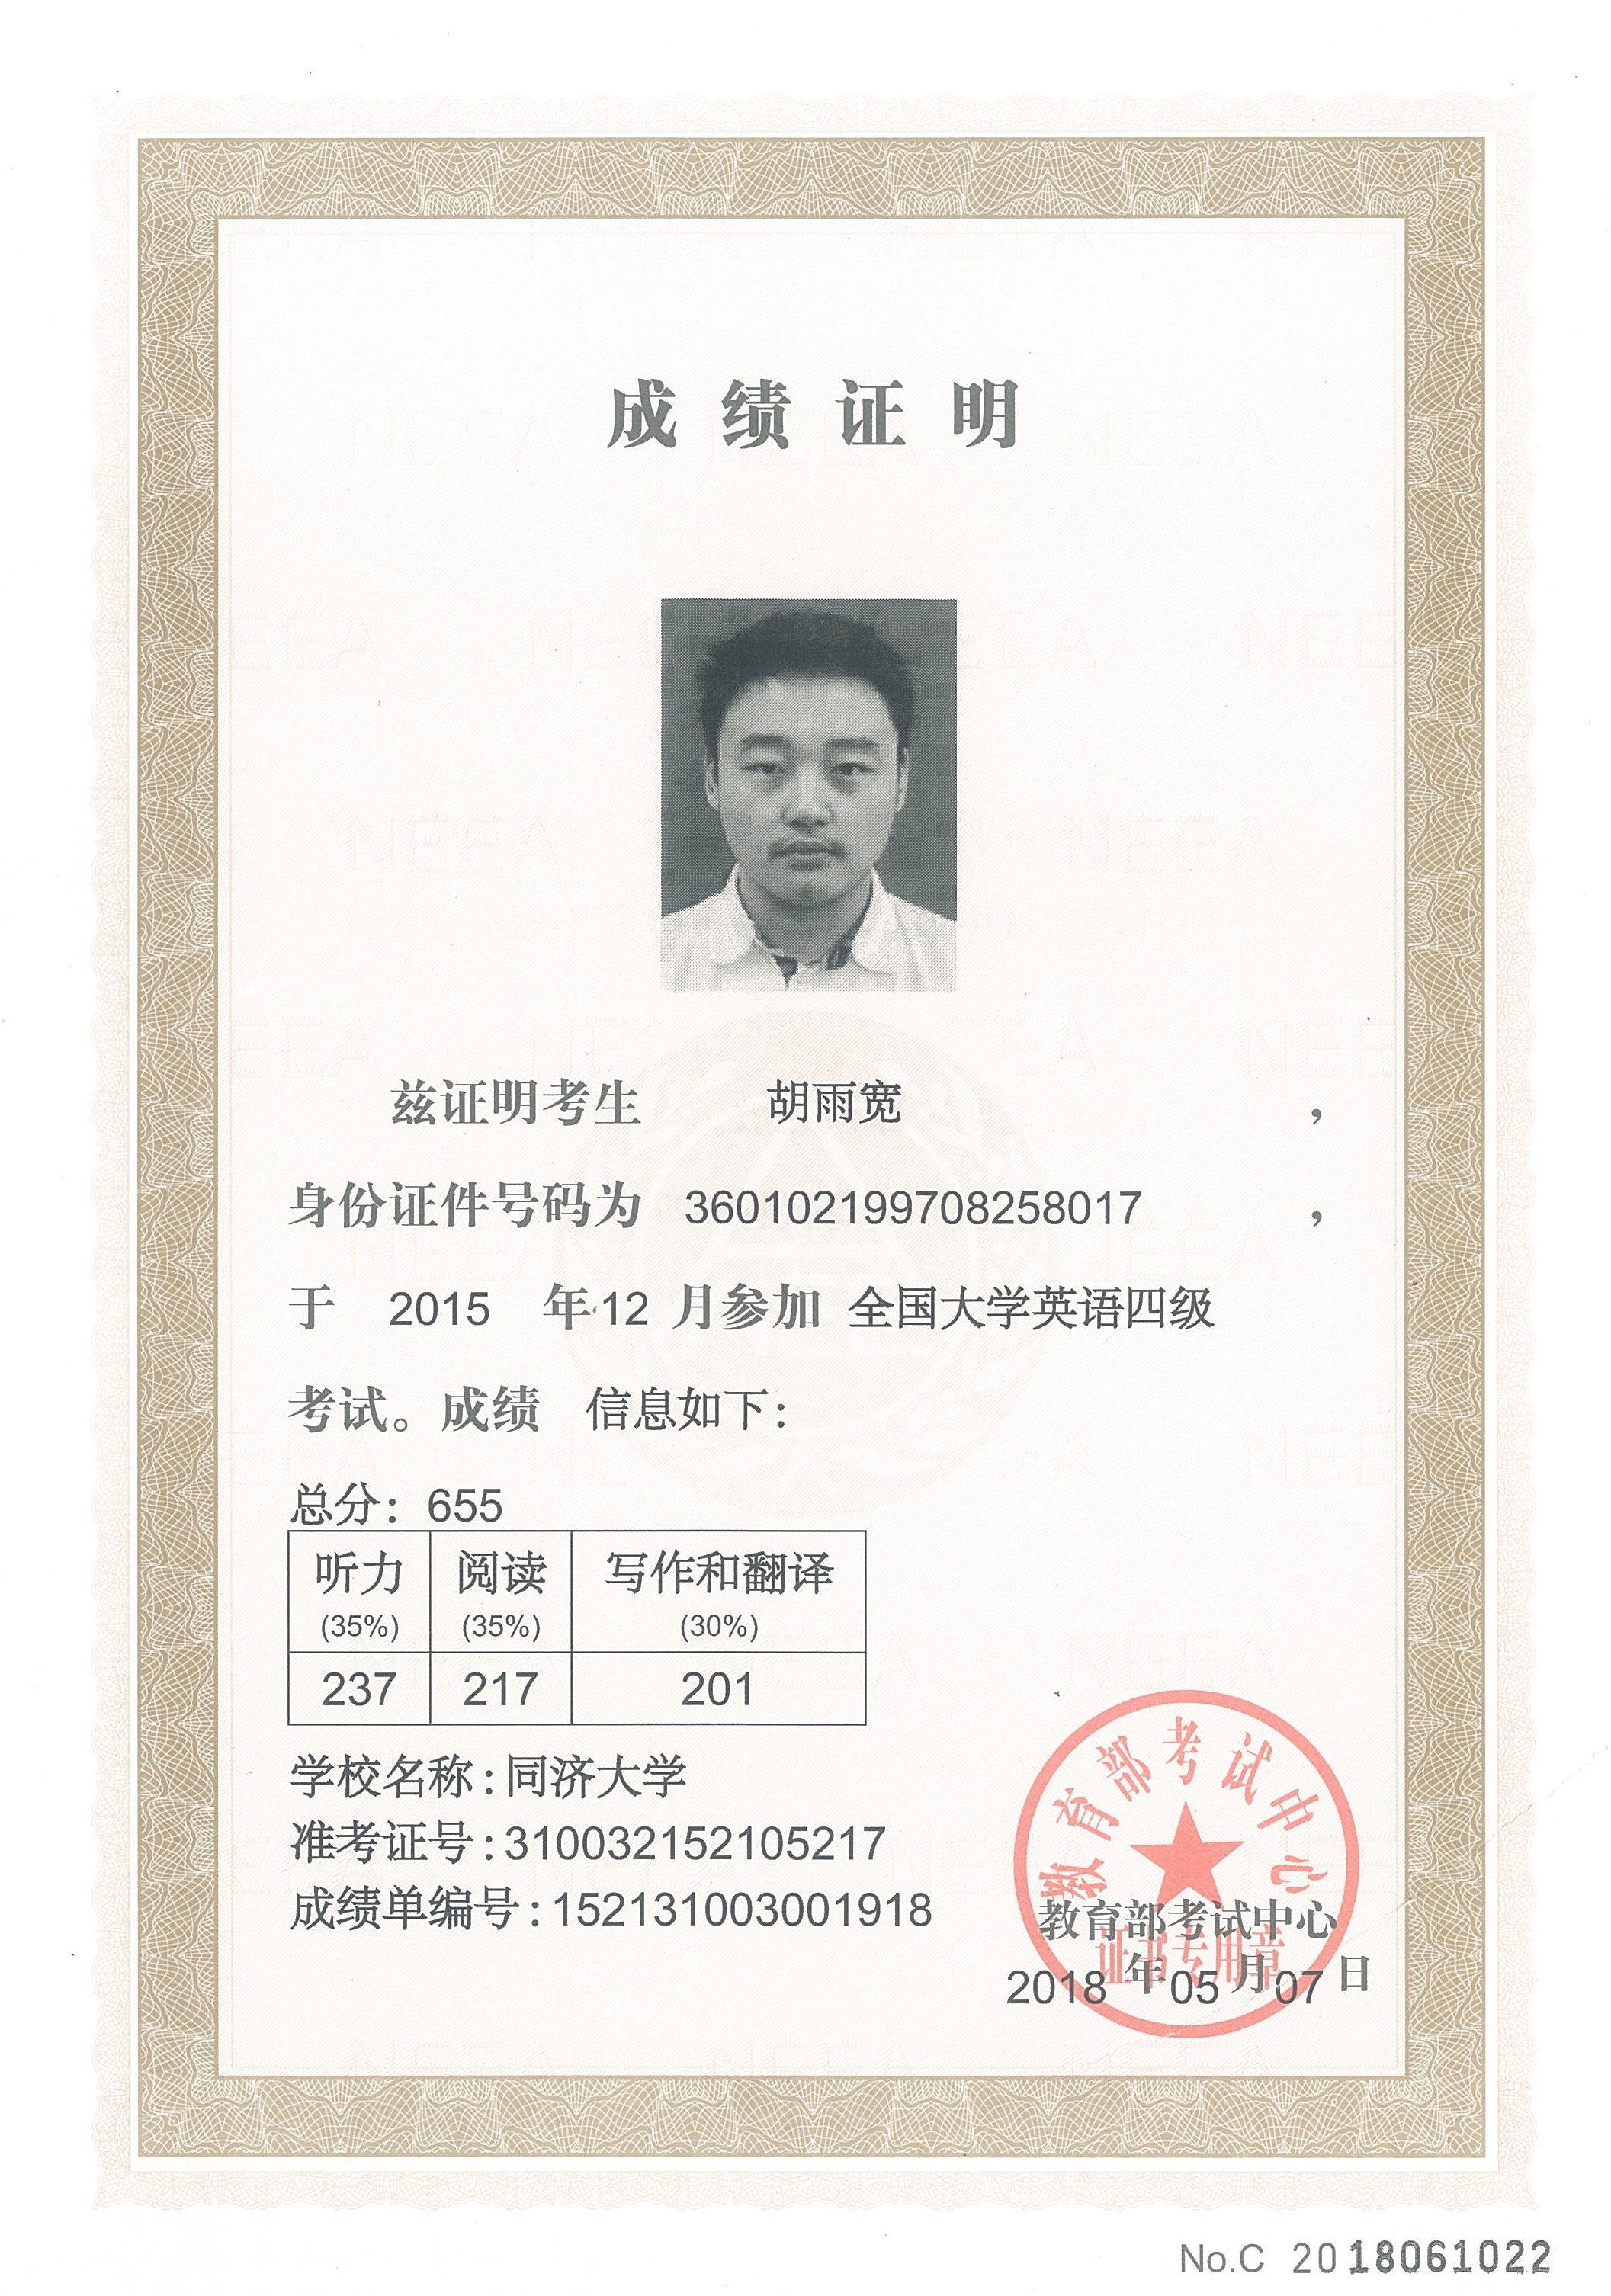
\includegraphics[height=3cm]{CET4.jpg}};
%  \node (img2) at (img1.south east) {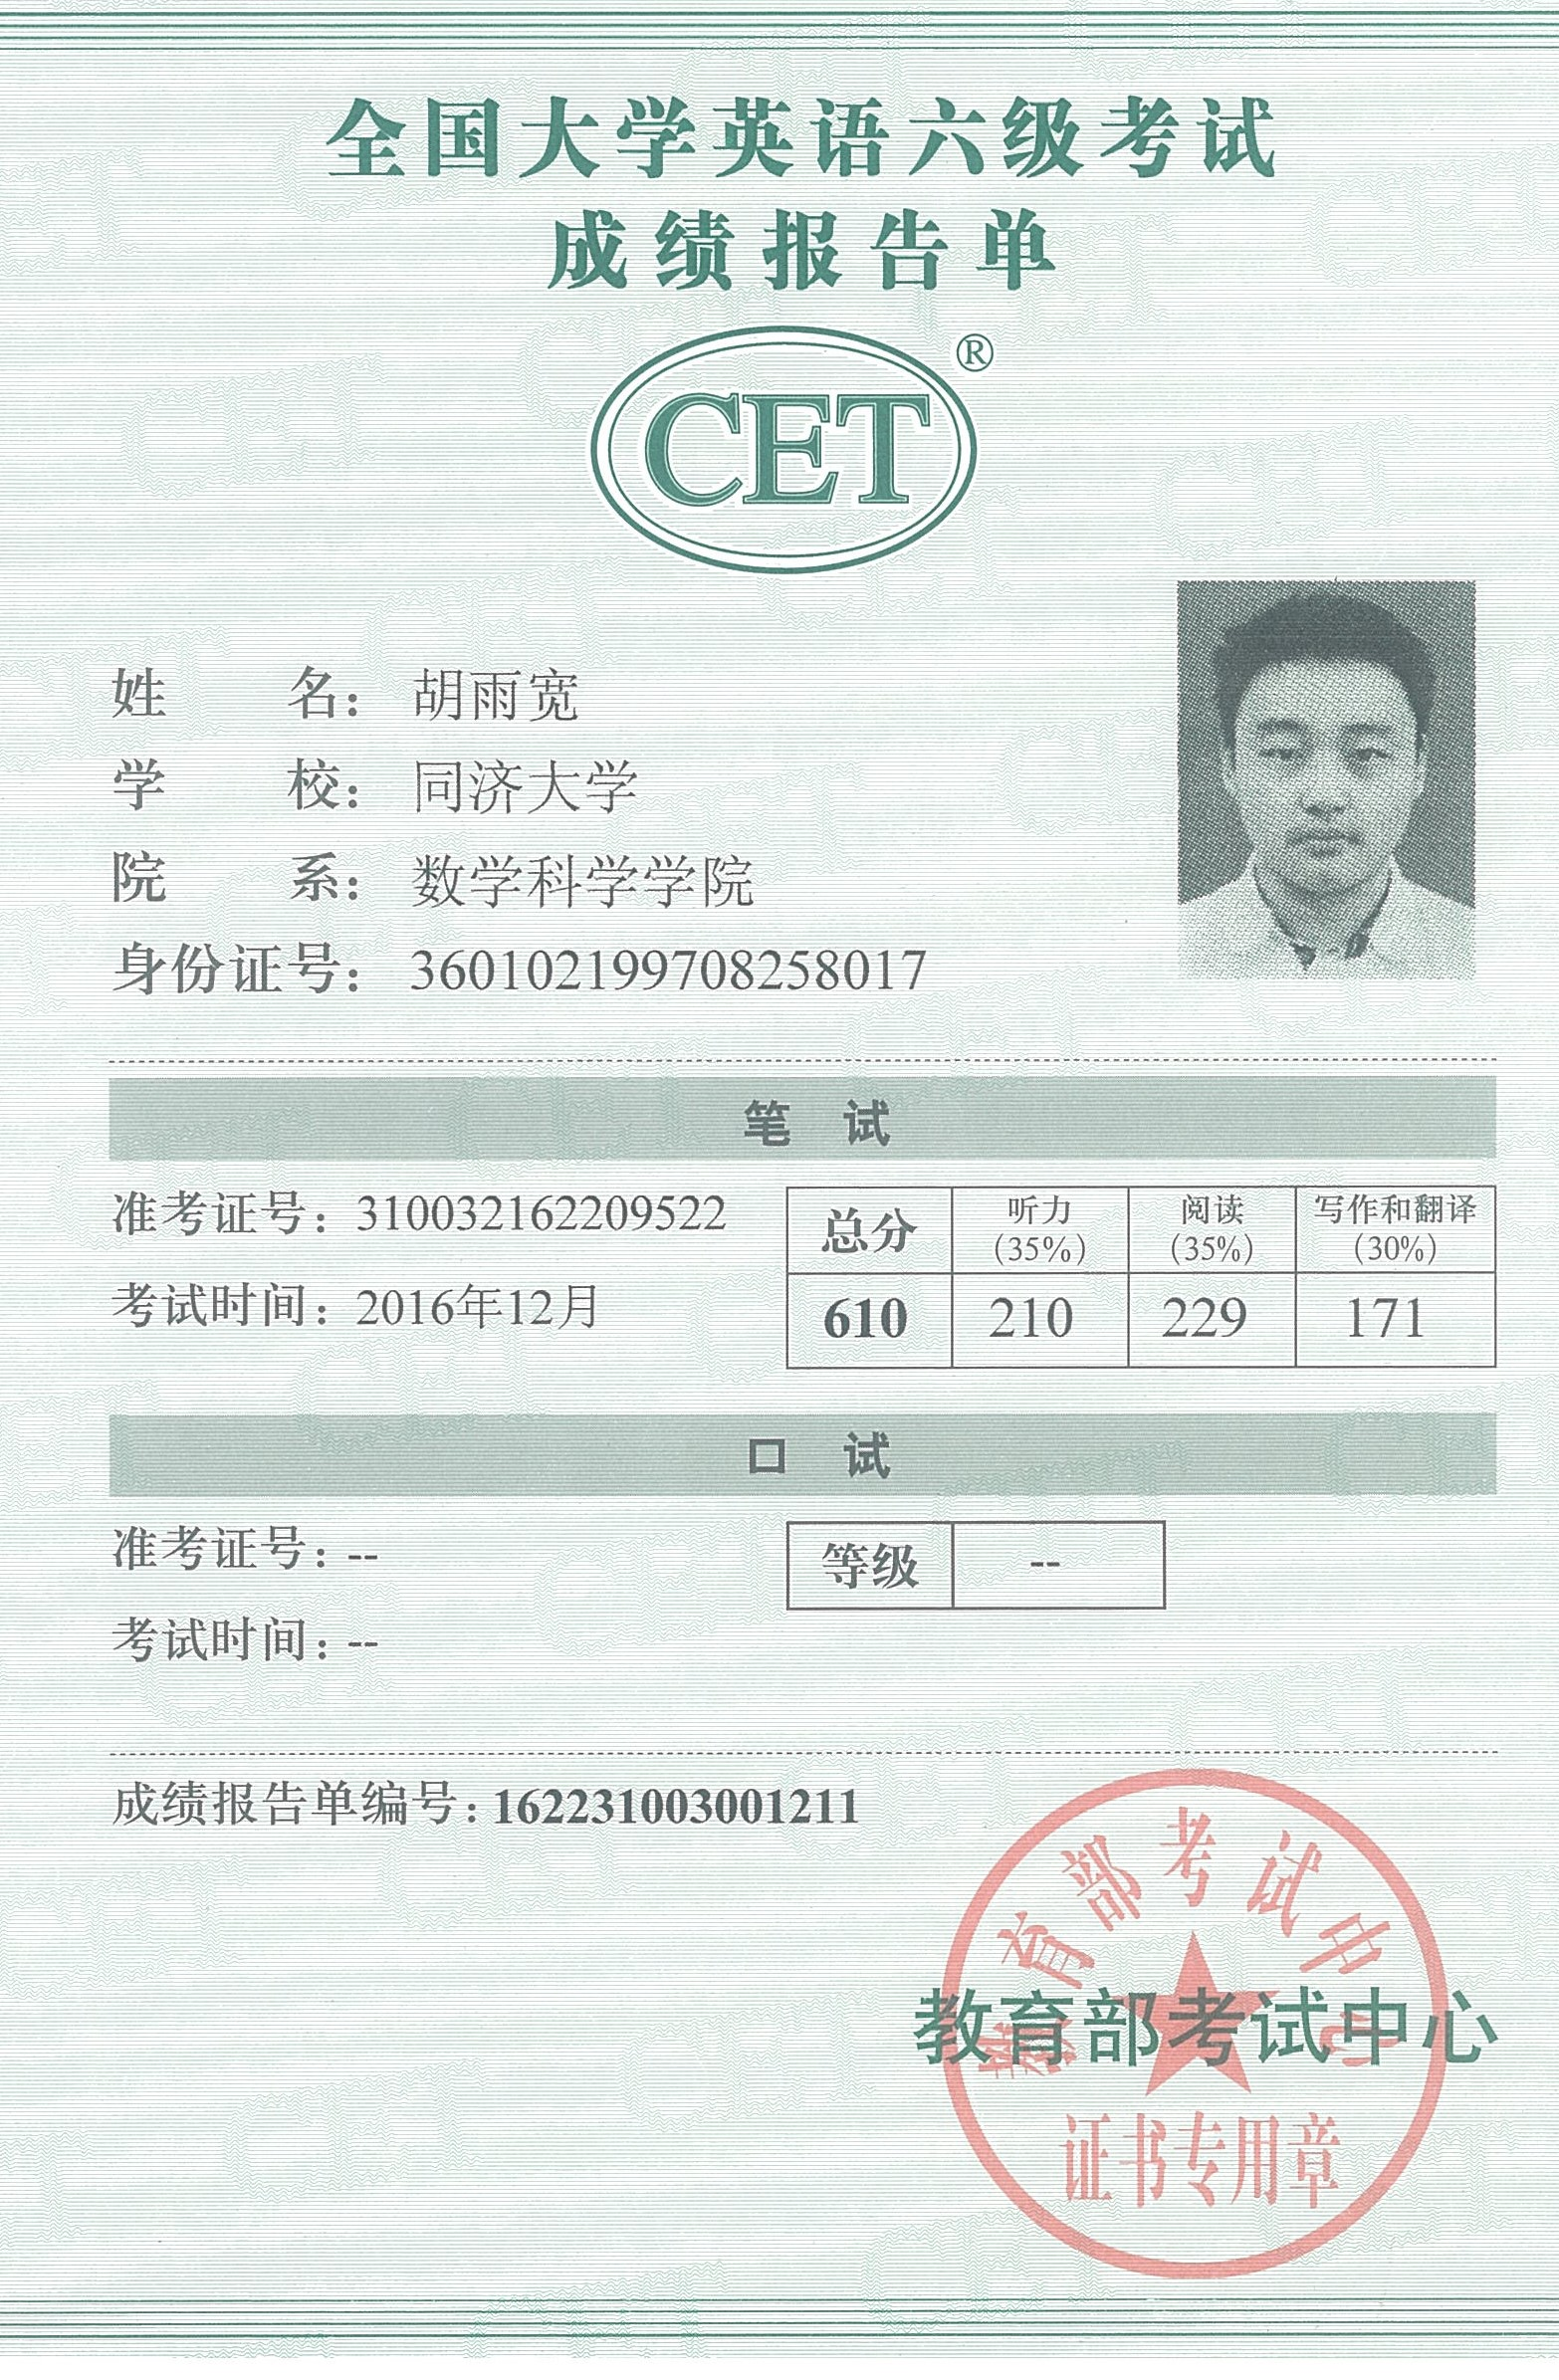
\includegraphics[height=3cm]{CET6.jpg}};
%\end{tikzpicture}
%\footnotesize \textbf{图}5: 外语成绩证明\end{center}
%}
%\end{column}
%\begin{column}{0.8\textwidth}
\begin{itemize}
\item 学习成绩: 7学期平均绩点4.85, {\color{red}{专业第二}}.\\
$\quad\quad\quad\quad\,$专业课绩点4.92.
\item 保研情况: 现已{\color{red}{保研至中国科学院数学与系统科学\\
$\quad\quad\quad\quad\,\,$研究院 (AMSS)}}, 方向为最优化计算.\\
$\quad\quad\quad\quad\,\,$硕博连读. {\color{red}{访问学者}} (2019.3-5).
\item 奖学金情况: {\color{red}连续3年获得本科生一等奖学金}.\\
$\quad\quad\quad\quad\quad\:\:$社会奖学金 (2017-2018).
\item 荣誉称号: ``优秀学生''称号 (2015-2016, 2017-2018).\\
$\quad\quad\quad\quad\:\:\:${\color{red}{``优秀学生标兵''称号 (2016-2017)}}.
\item 外语考试: CET4 655分,$\,${\color{red}{CET6 610分}}
\end{itemize}

%\end{column}
%\end{columns}
\end{frame}

\begin{frame}
\frametitle{学习方面——锐意进取$\,$开拓创新 (续)}
%\begin{columns}
%\begin{column}{0.3\textwidth}
%\only<2>{
%\begin{center}
%\begin{tikzpicture}
%  \node (img1) {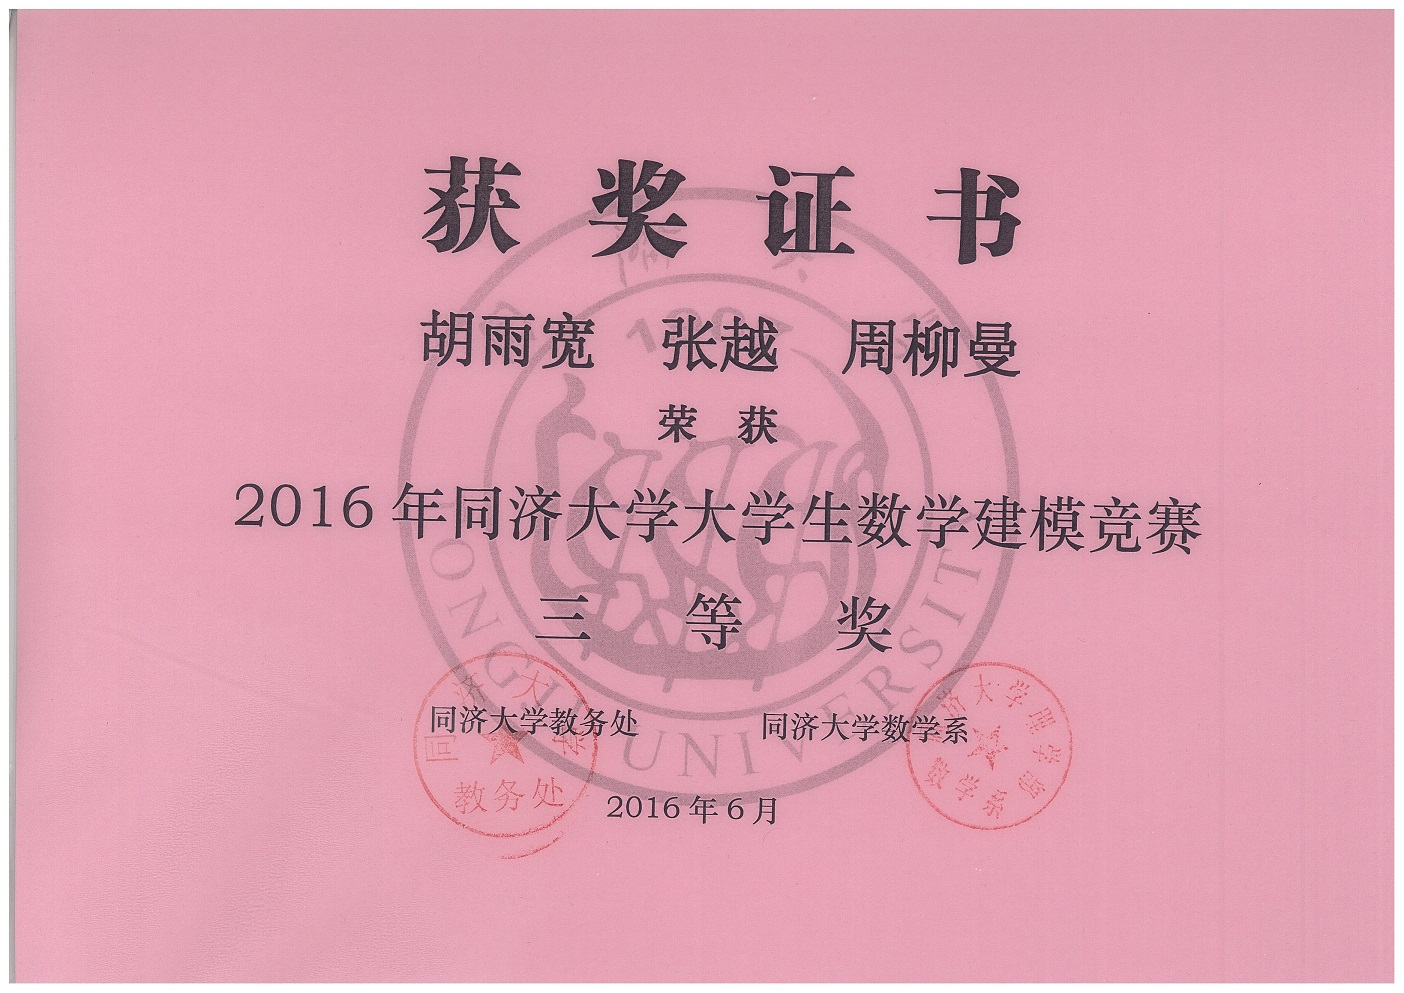
\includegraphics[height=2cm]{2016校赛建模三等奖.jpg}};
%  \node (img2) at (img1.south) {
\includegraphics[height=2cm]{2017校赛建模三等奖.jpg}};
%  \node (img3) at (img2.south) {
\includegraphics[height=2cm]{2018校赛建模三等奖.jpg}};
%\end{tikzpicture}
%\footnotesize \textbf{图}6: 数学建模竞赛 \\(校赛)\end{center}
%}
%\only<3>{
%\begin{center}
%\begin{tikzpicture}
%  \node (img1) {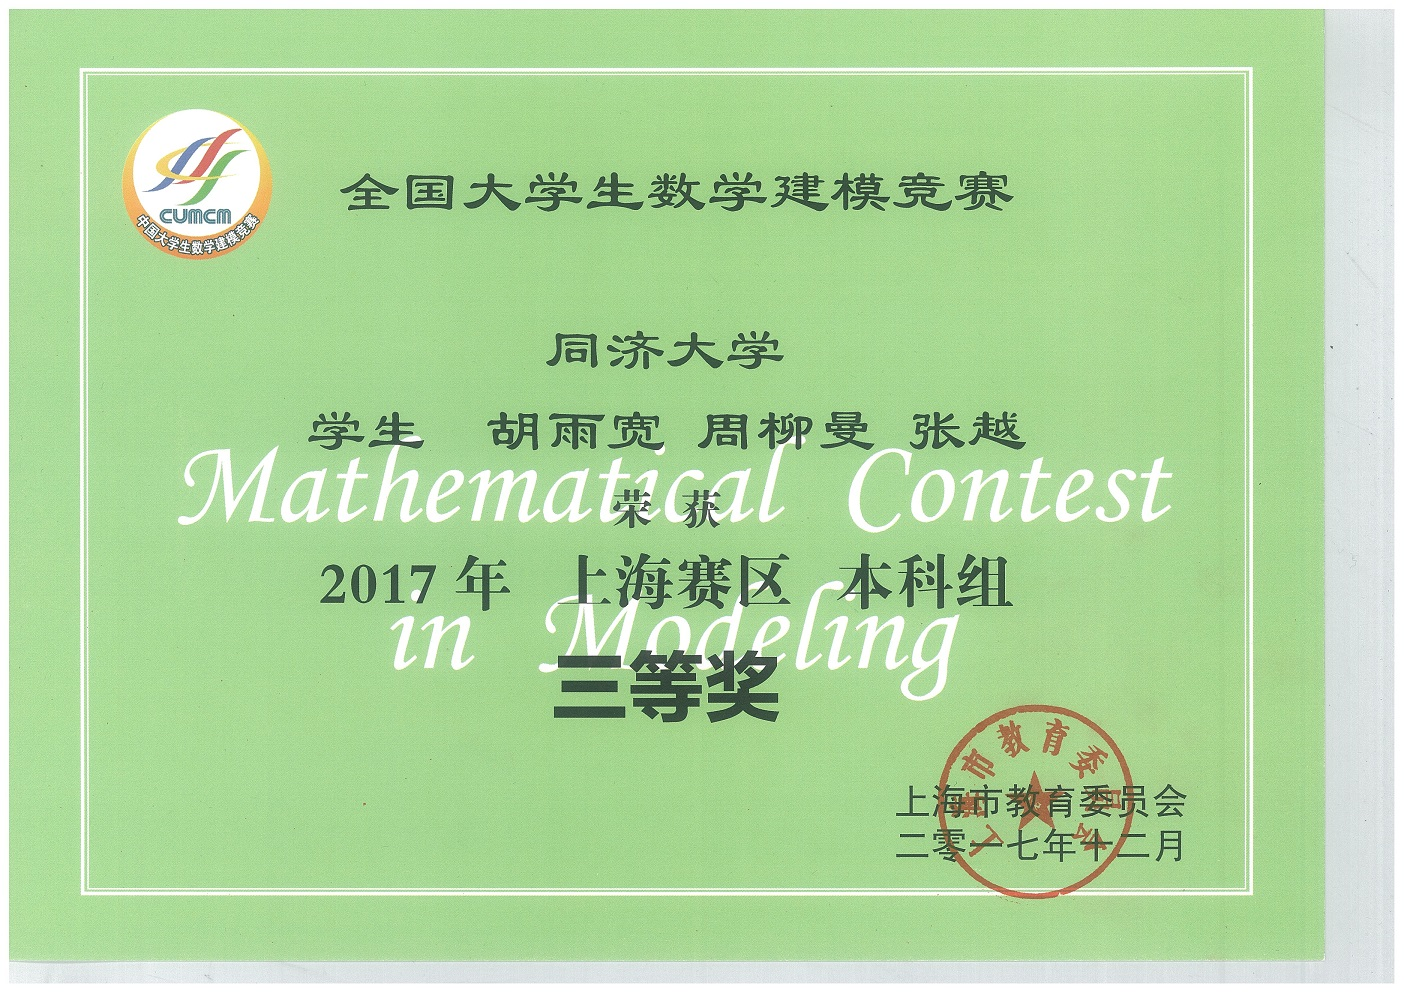
\includegraphics[height=2cm]{2017国赛建模三等奖.jpg}};
%  \node (img2) at (img1.south east) {
\includegraphics[height=2.5cm]{2018美赛二等奖.jpg}};
%\end{tikzpicture}
%\footnotesize \textbf{图}7: 数学建模竞赛\\ (国赛+美赛)
%\end{center}
%}
%\only<4>{
%\begin{center}
%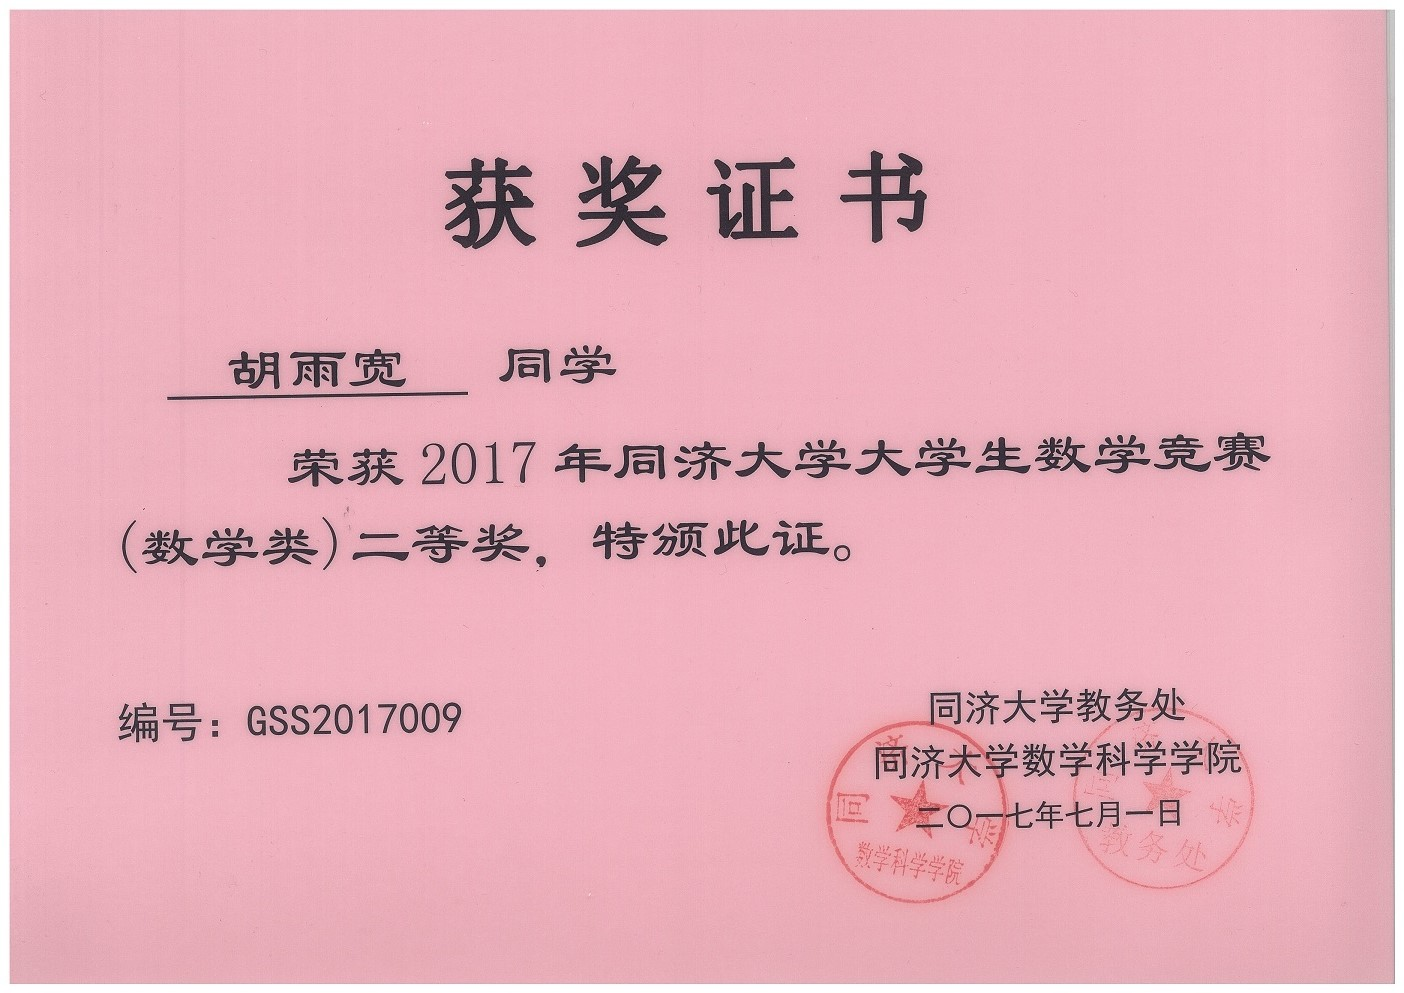
\includegraphics[width=3cm]{2017数学竞赛二等奖.jpg}\\
%\footnotesize \textbf{图}8: 数学竞赛
%\end{center}
%}
%\only<5>{
%\begin{center}
%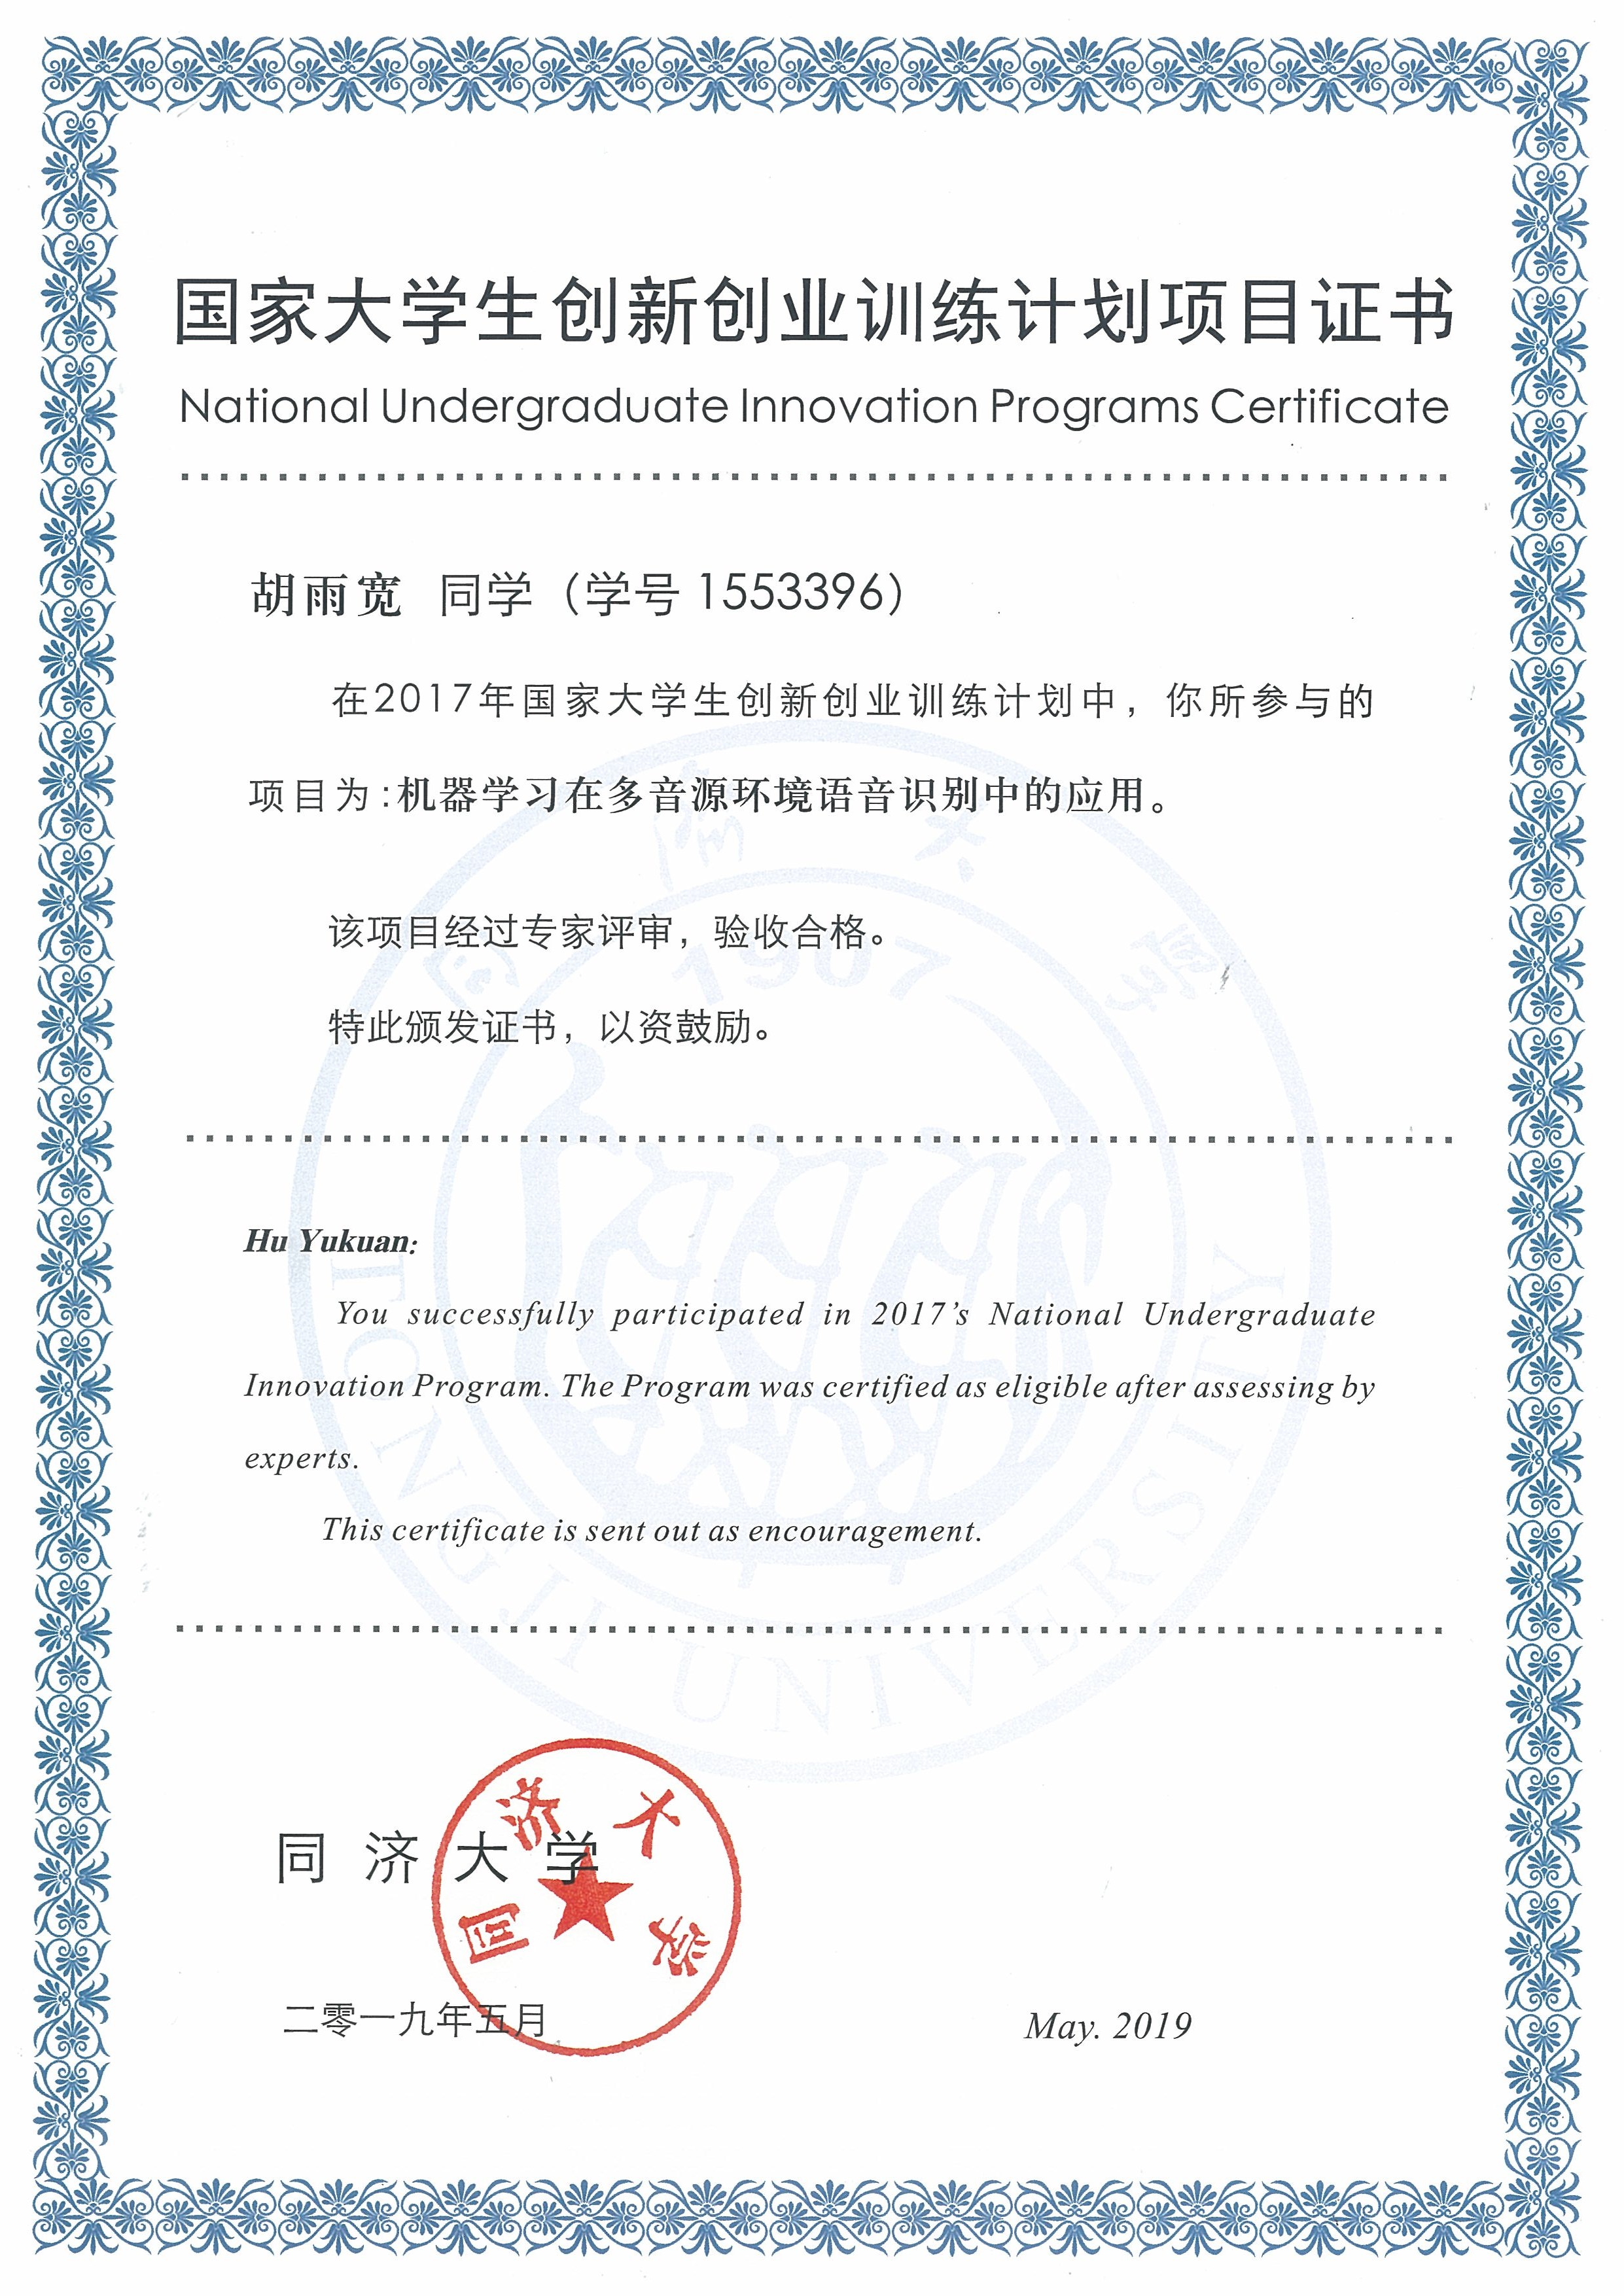
\includegraphics[width=3cm]{NIC.jpg}\\
%\footnotesize \textbf{图}9: 国创结题证书
%\end{center}
%}
%\end{column}
%\begin{column}{0.8\textwidth}
{\color{blue}{\textbf{科创竞赛}}}
\begin{itemize}
\item 数学建模: 校赛三等奖 (2016-2018, 团队, {\color{red}{队长}}).\\
$\quad\quad\quad\quad\:\:$国赛上海市三等奖 (2017, 团队, {\color{red}{队长}}).\\
$\quad\quad\quad\quad\:\:$美赛二等奖 (2018, 团队, {\color{red}{队长}}).
\item 数学竞赛: 校赛 (数学类)二等奖 (2017).
\item 创新项目: 机器学习在多音源环境语音识别中的应用\\
$\quad\quad\quad\quad\:\:\,\,$(2017.4-2019.4, {\color{red}{国创}}, {\color{red}{负责人}}, 已结题.)
\end{itemize}
%\end{column}
%\end{columns}
\end{frame}

\begin{frame}
\frametitle{学习方面——锐意进取$\,$开拓创新 (续)}
{\color{blue}{\textbf{科创竞赛}}}:\\
{\color{red}{2018年``浦发信用卡杯''中国高校SAS数据分析大赛全国总冠军, 我校历年\textbf{最好成绩} (团队, 队长).}}
\begin{figure}\centering
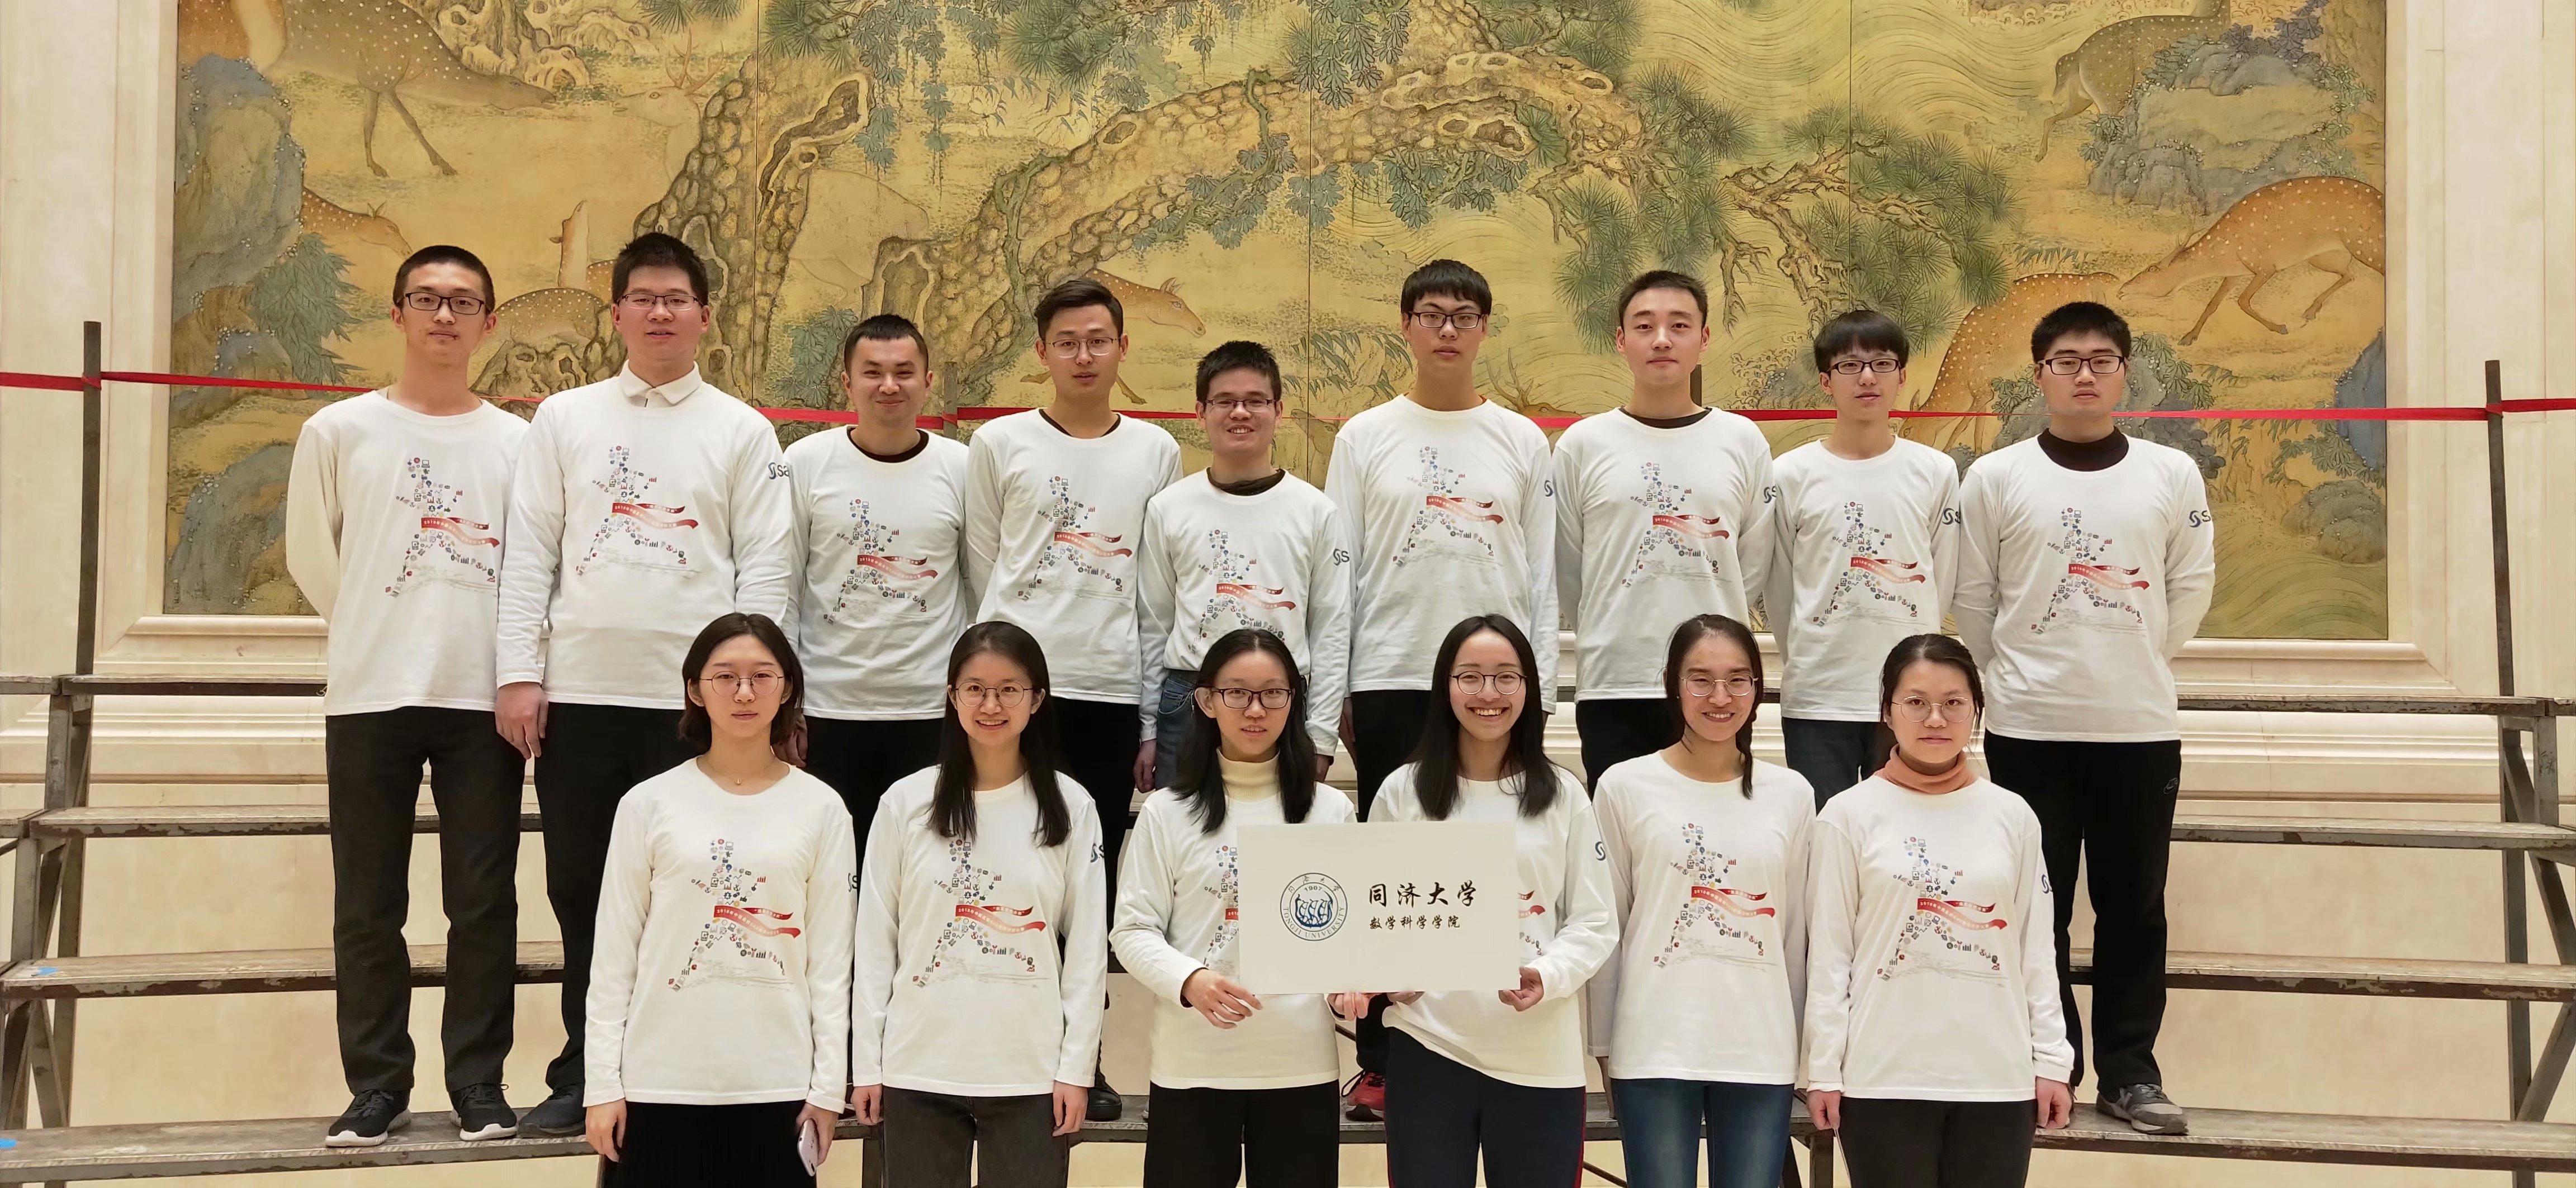
\includegraphics[width=.35\paperwidth]{SAStogether.jpg}$\quad$
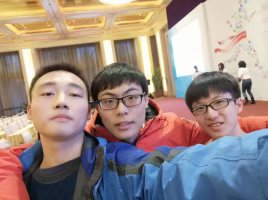
\includegraphics[width=.215\paperwidth]{SASphoto.jpg}\\\vspace{1em}

\includegraphics[width=.25\paperwidth]{SAScertificate.jpg}
\end{figure}
\begin{center}\footnotesize \textbf{图}1: 2018.11北京钓鱼台国宾馆颁奖现场\end{center}
\end{frame}

\section{实践与活动方面}
\begin{frame}
\frametitle{实践与活动方面——以身作则$\,$热心服务}
\onslide<1->{{\color{blue}{\textbf{学院层面}}}:}
\begin{itemize}
\item \onslide<2->{班级: 担任班长 (2018.4-至今).}
\item \onslide<2->{学生会: 学术部干事(2015.9-2017.9), ``光阴书会''.}
\item \onslide<2->{学院活动: 话剧比赛 (2016, 2018).\\
$\quad\quad\quad\quad\:\:$红歌会 (2017). \\
$\quad\quad\quad\quad\:\:$晚会 (2015, 2018).}
\item \onslide<2->{{\color{red}{当选同济大学第四十二次学代会的学生代表和数学科学学院常代表 (2018)}}.}
\end{itemize}
\end{frame}

\begin{frame}
\frametitle{实践与活动方面——以身作则$\,$热心服务 (续)}
\onslide<1->{{\color{blue}{\textbf{学院层面}}}:}\\
\onslide<1->{学生组织: 加入{\color{red}{``数学外卖''活动}}, 进入线性代数组 (2017.6).\\
$\quad\quad\quad\quad\:\:$担任线性代数组{\color{red}{组长}} (2018.4-至今).\\
\onslide<2->{$\quad\quad\:\:$1. 制作参考课件, 统一课件样式;\\
$\quad\quad\:\:$2. 充分利用组内资源, 鼓励新人上场, 任期内3场讲座、1次辅导\\
$\quad\quad\:\:$3. 完善相关制度.}\\[1em]
个人累计3场讲座、3次辅导. {\color{red}{``金牌讲师''}}. \\
{\color{red}{``2017-2018年优秀志愿服务项目''}}.}
\begin{center}
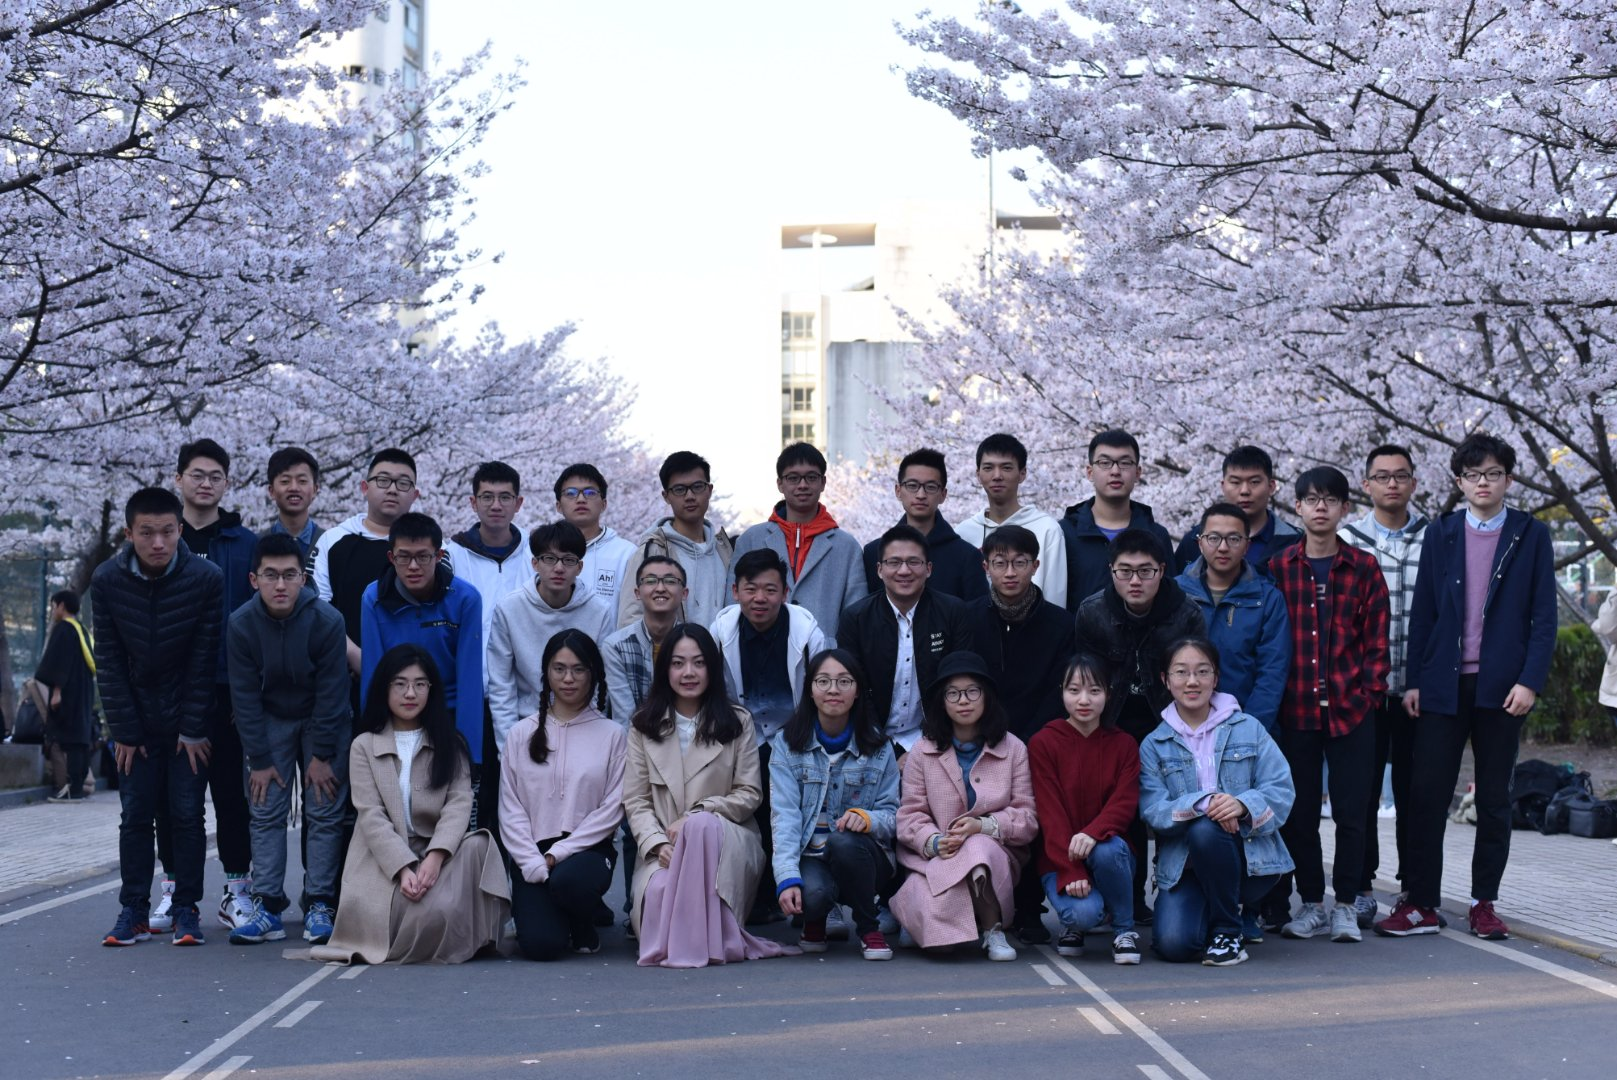
\includegraphics[width=.3\paperwidth]{linearalgebra.jpg}$\quad$
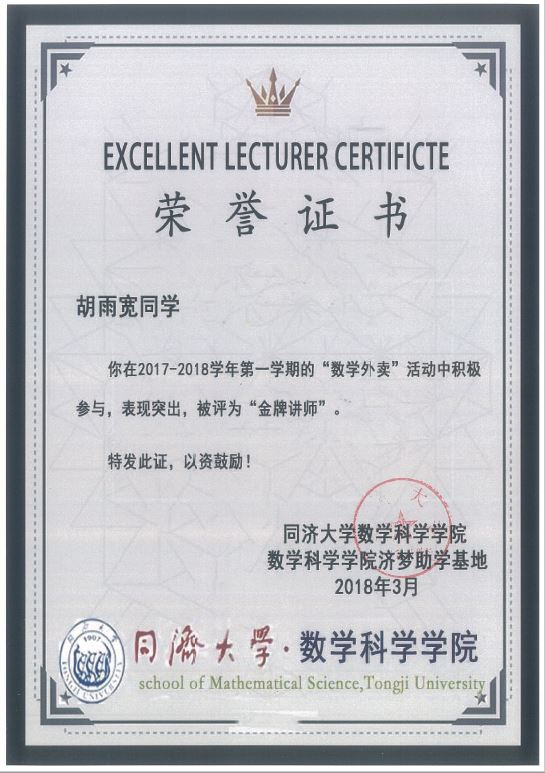
\includegraphics[width=.15\paperwidth]{gold.jpg}$\quad$

\includegraphics[width=.28\paperwidth]{slide.png}\\
\footnotesize \textbf{图}2: 左: ``全''家福; 中: ``金牌讲师''; 右: 课件一页
\end{center}
\end{frame}

\begin{frame}
\frametitle{实践与活动方面——以身作则$\,$热心服务 (续)}
\onslide<1->{{\color{blue}{\textbf{学校层面}}}:}\\
\onslide<1->{志愿服务: 义务献血(2015, 2016, 2017, 2018).} 
\only<1>{\\$\quad\quad\quad\quad\:\:\,\,$110周年校庆志愿者活动 (2017).}
\only<2>{{\\\color{red}{$\quad\quad\quad\quad\:\:\,\,$110周年校庆志愿者活动 (2017).}}}
\only<3->{\\$\quad\quad\quad\quad\:\:\,\,$110周年校庆志愿者活动 (2017).}
\only<1-2>{\\$\quad\quad\quad\quad\:\:$迎新生``小红帽''志愿者活动 (2018).}
\only<3->{{\\\color{red}{$\quad\quad\quad\quad\:\:$迎新生``小红帽''志愿者活动 (2018).}}}
\only<2>{\begin{center}
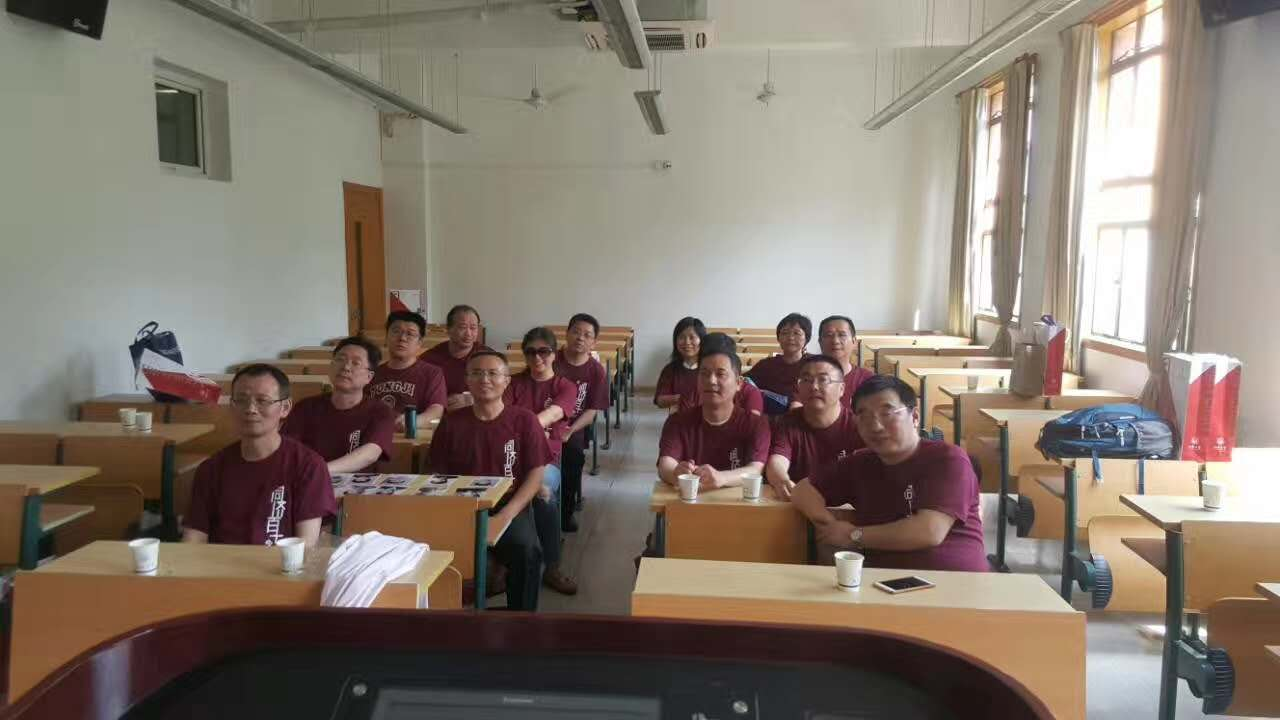
\includegraphics[width=.6\paperwidth]{520.jpg}\\
\footnotesize\textbf{图}3: 2017.5.20 我院1985级校友合影
\end{center}}
\onslide<3->{\begin{center}
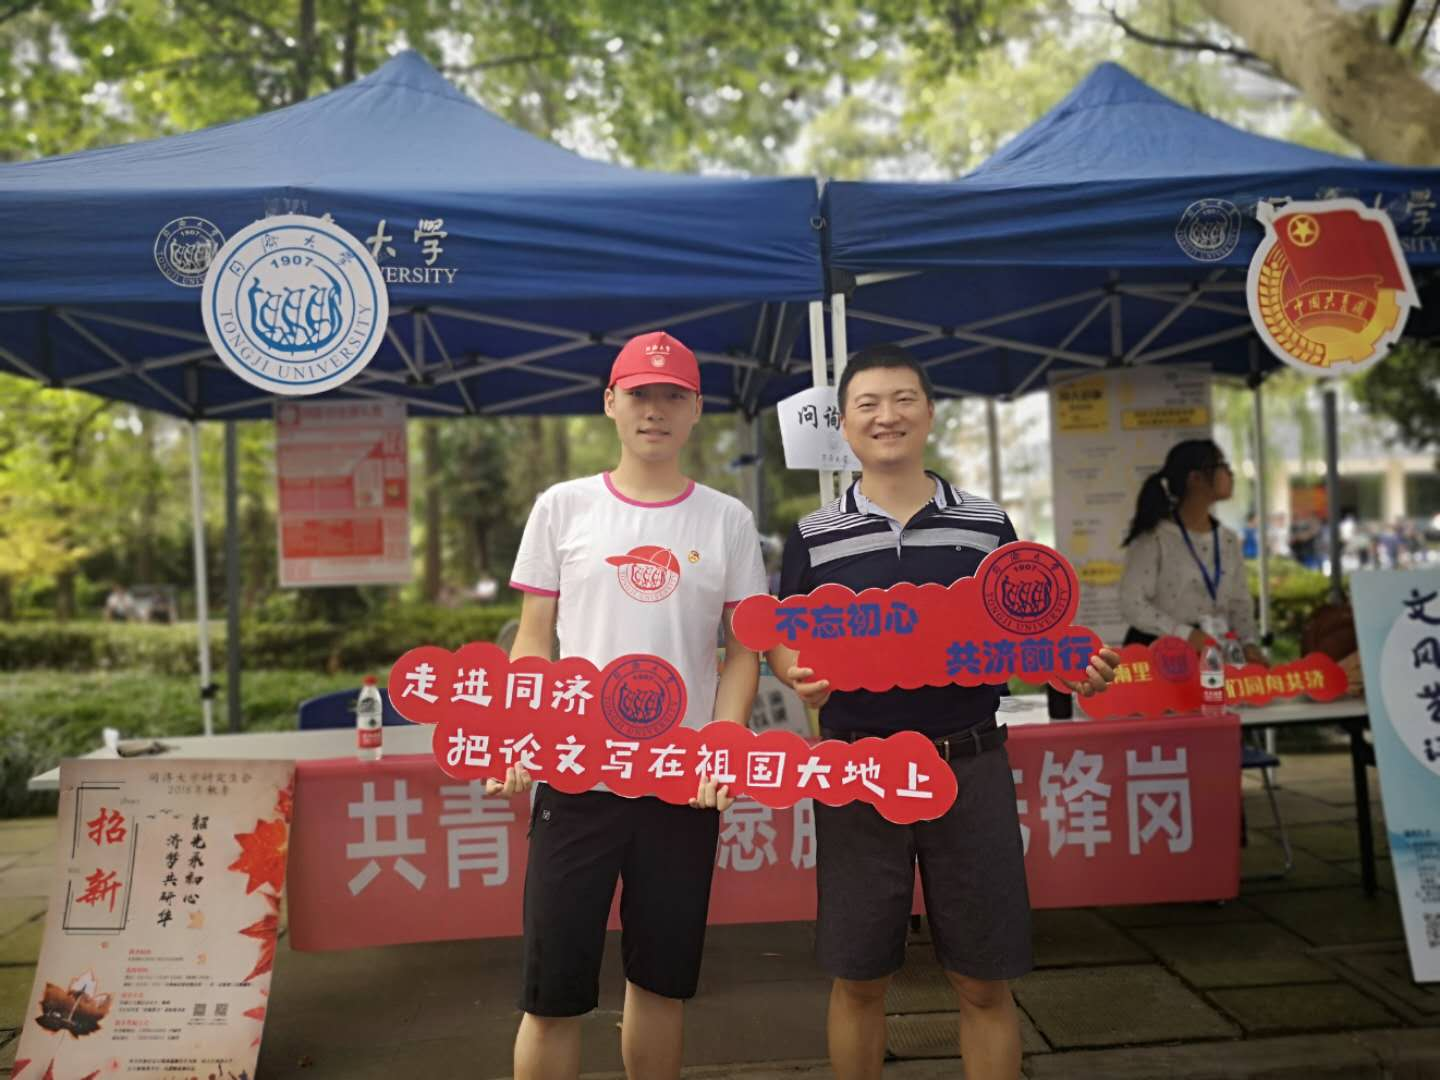
\includegraphics[width=.415\paperwidth]{redhat1.jpg}$\:$
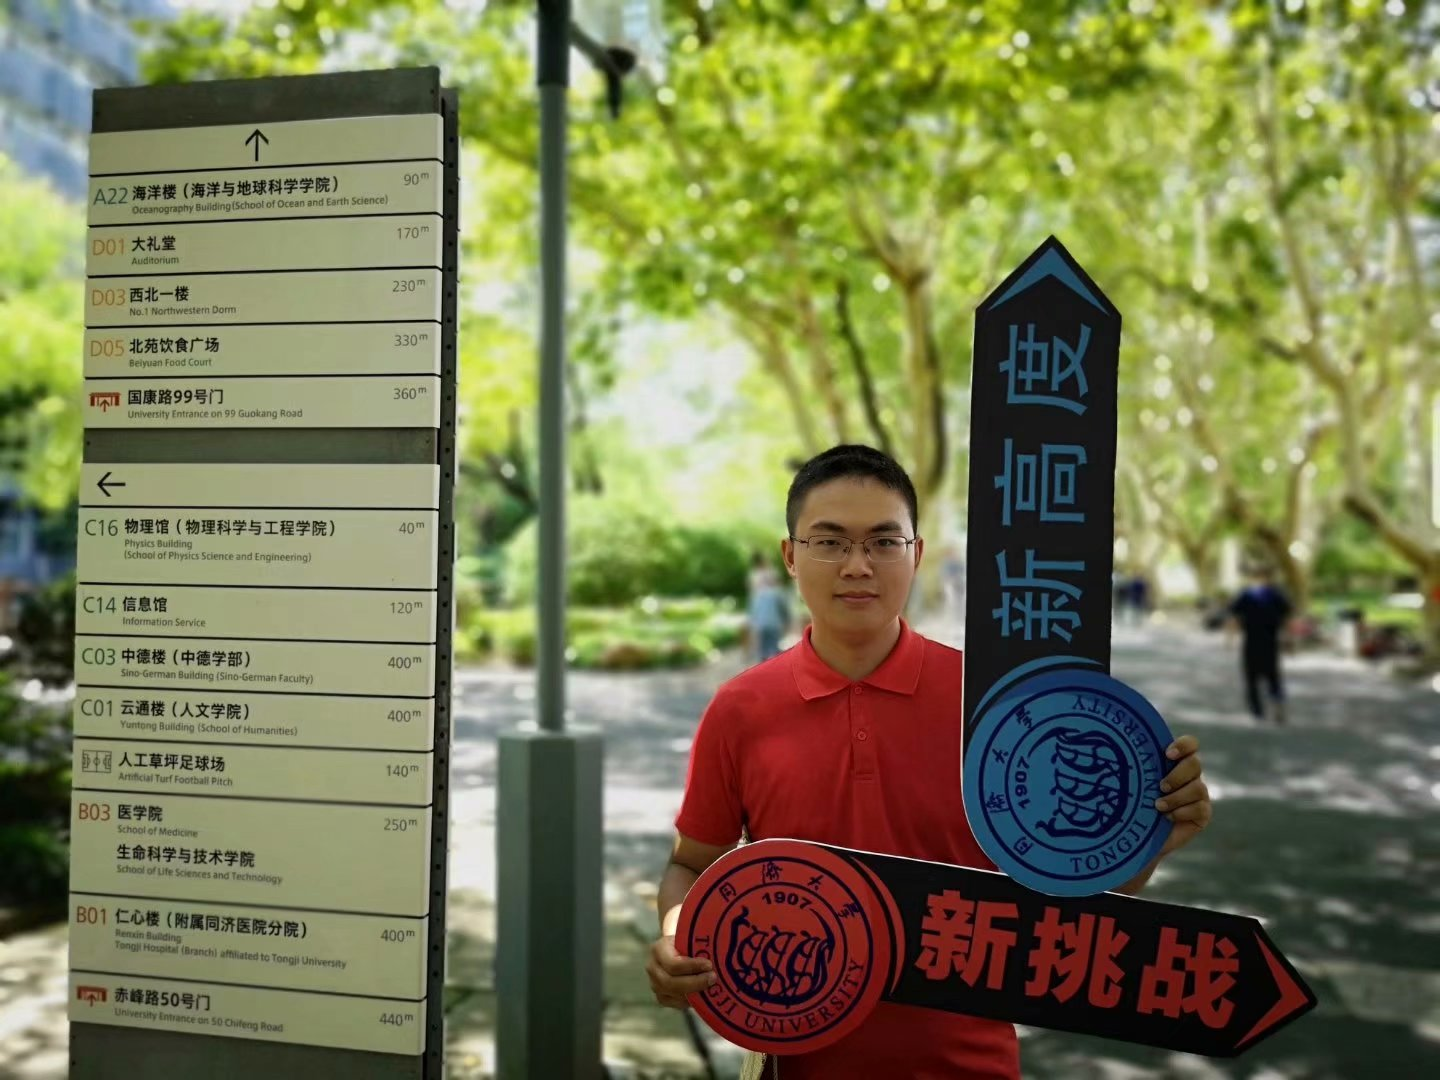
\includegraphics[width=.415\paperwidth]{redhat2.jpg}\\
\footnotesize \textbf{图}4: 2018.9 ``小红帽''活动\end{center}}
\end{frame}

\section{其他方面}
\begin{frame}
\frametitle{其他方面——全面发展$\,$持之以恒}
{\color{blue}{\textbf{体育锻炼}}}: \pause 长跑 (3km$\to$5km$\to$8km$\to$10km$\to$20km), 定协\pause
\begin{itemize}
\onslide<3->{\item 2018北京马拉松线上赛 (10km, {\color{red}{完赛}}成绩50分58秒, 第411名)}
\onslide<4->{\item 2018广州马拉松线上赛 (10km, {\color{red}{完赛}}成绩44分59秒)}
\onslide<5->{\item 2019扬州半程马拉松线上赛 (半程21.0975km, {\color{red}{完赛}}成绩1小时58分02秒)}
\end{itemize}

\begin{center}\onslide<3->{
\includegraphics[width=.16\paperwidth]{bjmarathon.jpg}}$\quad$
\onslide<4->{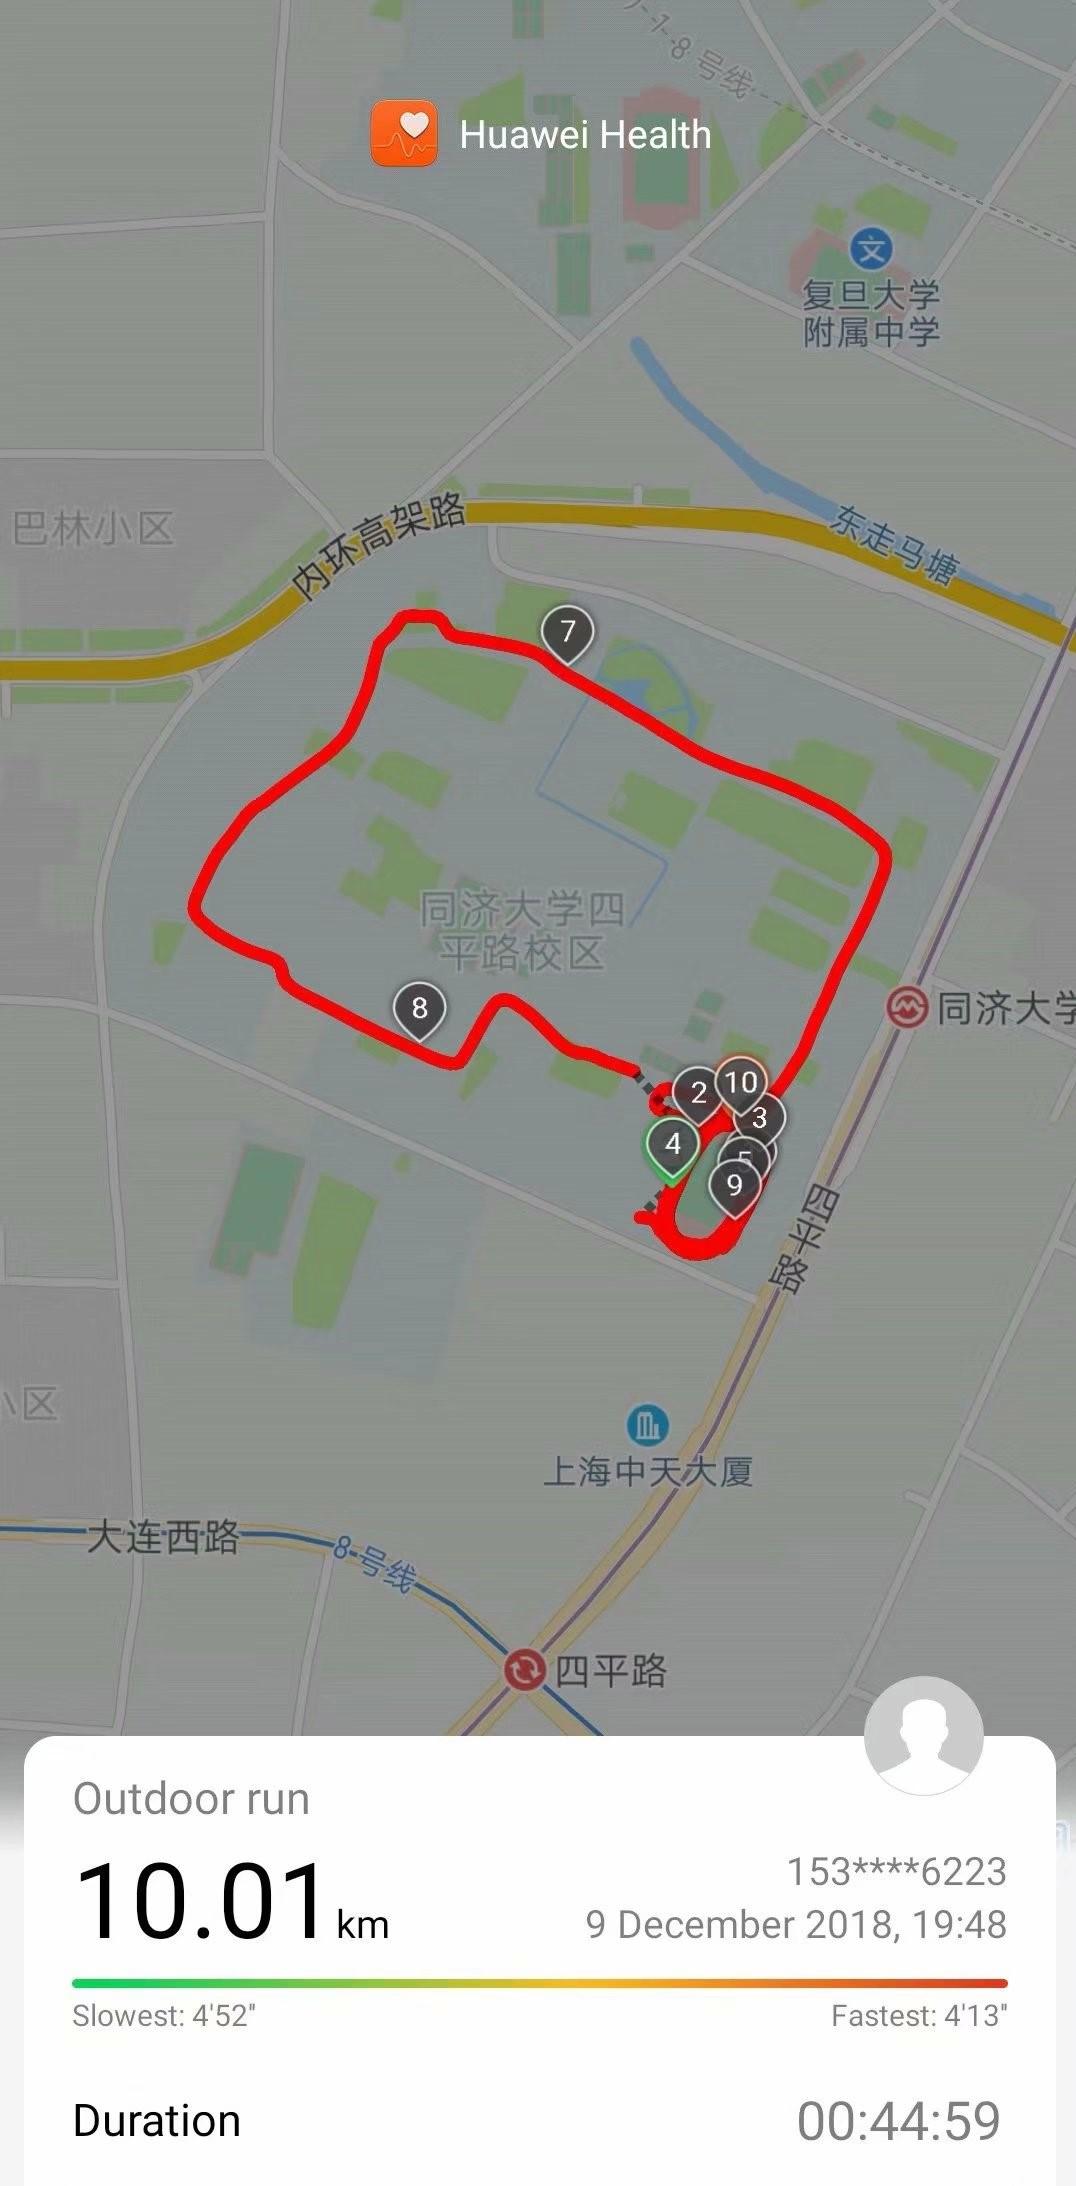
\includegraphics[width=.165\paperwidth]{gzmarathon.jpg}}$\quad$
\onslide<5->{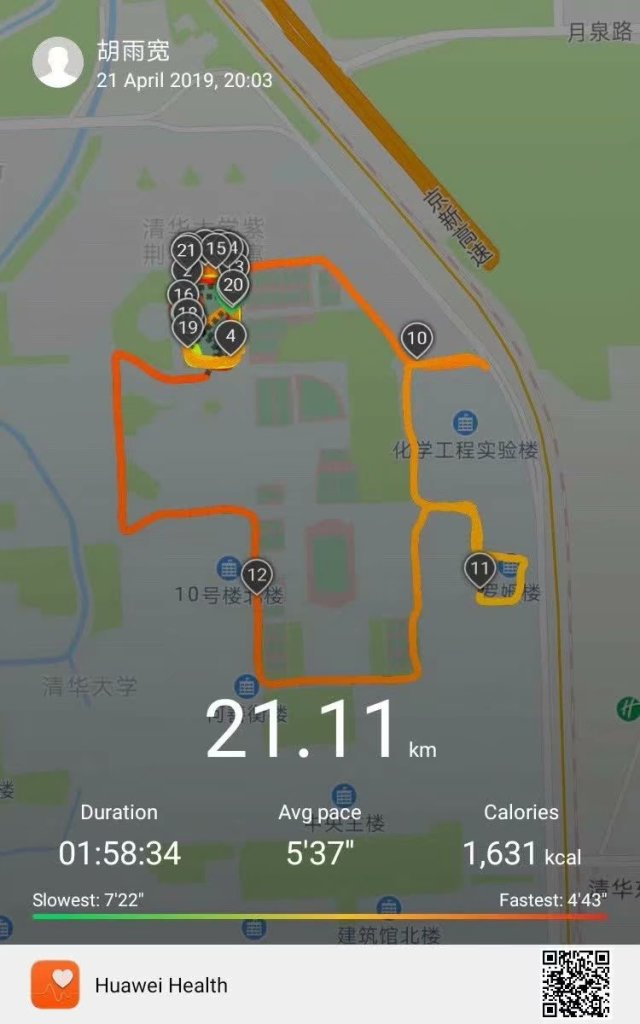
\includegraphics[width=.21\paperwidth]{yzmarathon.jpg}}\\
\footnotesize \onslide<5->{\textbf{图}5: 马拉松线上赛成绩截图}\end{center}
\end{frame}

\begin{frame}
\frametitle{其他方面——全面发展$\,$持之以恒 (续)}
{\color{blue}{\textbf{学校比赛}}}
\begin{itemize}
\item 健美操比赛团体一等奖 (2015, 2016).
\item 同济大学第二届``体质达人''比赛``肺活量''和``身体成分''组双料``体质达人'' (2017).
\end{itemize}
\end{frame}

\begin{frame}{致谢}
\begin{center}
\huge \songti 感谢聆听!\\[0.3em]
\normalsize
\url{huyukuan2015@tongji.edu.cn}
\end{center}
\end{frame}

\end{document}


